\section{CP from eigenvalues} % {{{
% Intro {{{
Choi matrix's eigenvalues of a 1-qubit Pauli Channel are
\begin{align}
\lambda_{\mu}=1+\sum_{j=1}^3a_j^{\mu}\tau_j
\hspace{35pt}
\mu=0,1,2,3;
\hspace{35pt}
a_j^{\mu}=\left\{ \begin{array}{rl}
             1, & \mu=j \lor \mu=0\\
             -1, & \mu\neq j
             \end{array}
   \right..
\end{align}
Therefore, the inequalities needed to be sattisfied for a 1-qubit 
unital Pauli channel in order to be CP may be expressed in the 
following compact expression:
\begin{equation}
\sum_{j=0}^3a_j^{\mu}\tau_j\geq -1,
\hspace{35pt}
\mu=1,2,3;
\hspace{35pt}
a_j^{\mu}=\left\{ \begin{array}{rl}
             1, & \mu=j\\
             -1, & \mu\neq j
             \end{array}
   \right..
\end{equation}

Now, Choi matrix's eigenvalues of an n-qubit Pauli Channel are
\begin{align}\label{eq:eigvals-PCE}
\lambda_{\mu_1,\ldots,\mu_n}=1+
\sum_{\underset{(j_1,\ldots,j_n\neq0)}{j_1,\ldots,j_n=0}}^3
a_{j_1}^{\mu_1}\ldots a_{j_n}^{\mu_n}\tau_{j_1,\ldots,j_n}
\hspace{35pt}
\mu_l&=0,1,2,3,\nonumber\\
a_{j_l}^{\mu_l}&=\left\{ \begin{array}{rl}
             1, & \mu_l=j_l \lor j_l=0\lor \mu_1,\ldots,\mu_n=0\\
             -1, & \mu_l\neq j_l
             \end{array}
   \right..
\end{align}

Therefore, the inequalities needed to be sattisfied for the CP are
\begin{equation}\label{eq:inequalities-PCE}
\sum_{\underset{(j_1,\ldots,j_n\neq0)}{j_1,\ldots,j_n=0}}^3
a_{j_1}^{\mu_1}\ldots a_{j_n}^{\mu_n}\tau_{j_1,\ldots,j_n}
\geq
-1,
\hspace{35pt}
\mu_l=0,1,2,3;
\hspace{35pt}
a_{j_l}^{\mu_l}=\left\{ \begin{array}{rl}
             1, & \mu_l=j_l \lor j_l=0\\
             -1, & \mu_l\neq j_l
             \end{array}
   \right.,
\end{equation}
where we used that $\lambda_{0,\ldots,0}$ is always non-negative.
% }}}
\subsection{Another observation from this} % {{{
Choi's matrix of 2 qubits is diagonal in Pauli product basis
(Kraus operators). Does this follow in the general case???? 
% }}}
% }}}
\section{General characterisation of PCE quantum channels} % {{{
\subsubsection*{To avoid confusion} % {{{
\cpnote{Igual el canal totalmente despolarizante y el estado totalmente mixto 
tendrían el mismo diagrama. Quiza el borde se puede ser de diferente color
}
\janote{Me gustaría discutir antes si igual vale la pena hacer la distinción.
Dado que al final la distinción sólo es una ayuda que se me ocurrió para 
explicar gráficamente el procedimiento de la concatenación.}
The figures we've been using (columns, boards, cubes) may represent
both PCE operations (dynamics) and density matrices (kinematics). We
will make a distinction between both representations with colors.
B$\&$W represent PCE operations, and colored figures represent 
density matrices in Pauli products basis.
\begin{figure}[H]
\begin{subfigure}{.5\textwidth}
\centering
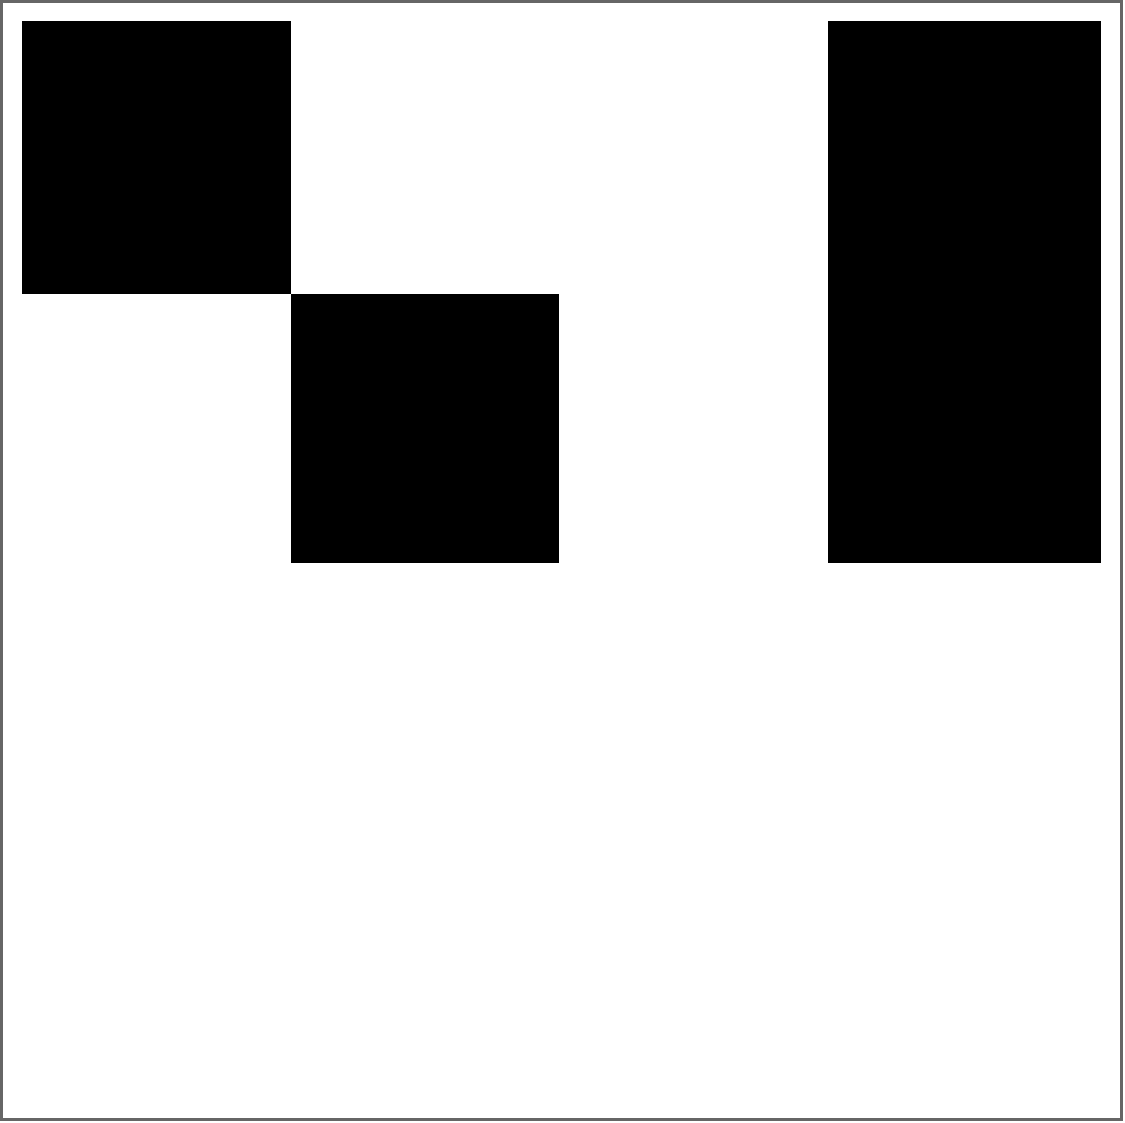
\includegraphics[width=3cm]{PCEoperation}
\caption{PCE operation that erases all Pauli components except 
for $r_{0,0}$, $r_{1,1}$, $r_{1,3}$, and $r_{0,3}$.}
\end{subfigure}
\begin{subfigure}{.5\textwidth}
\centering
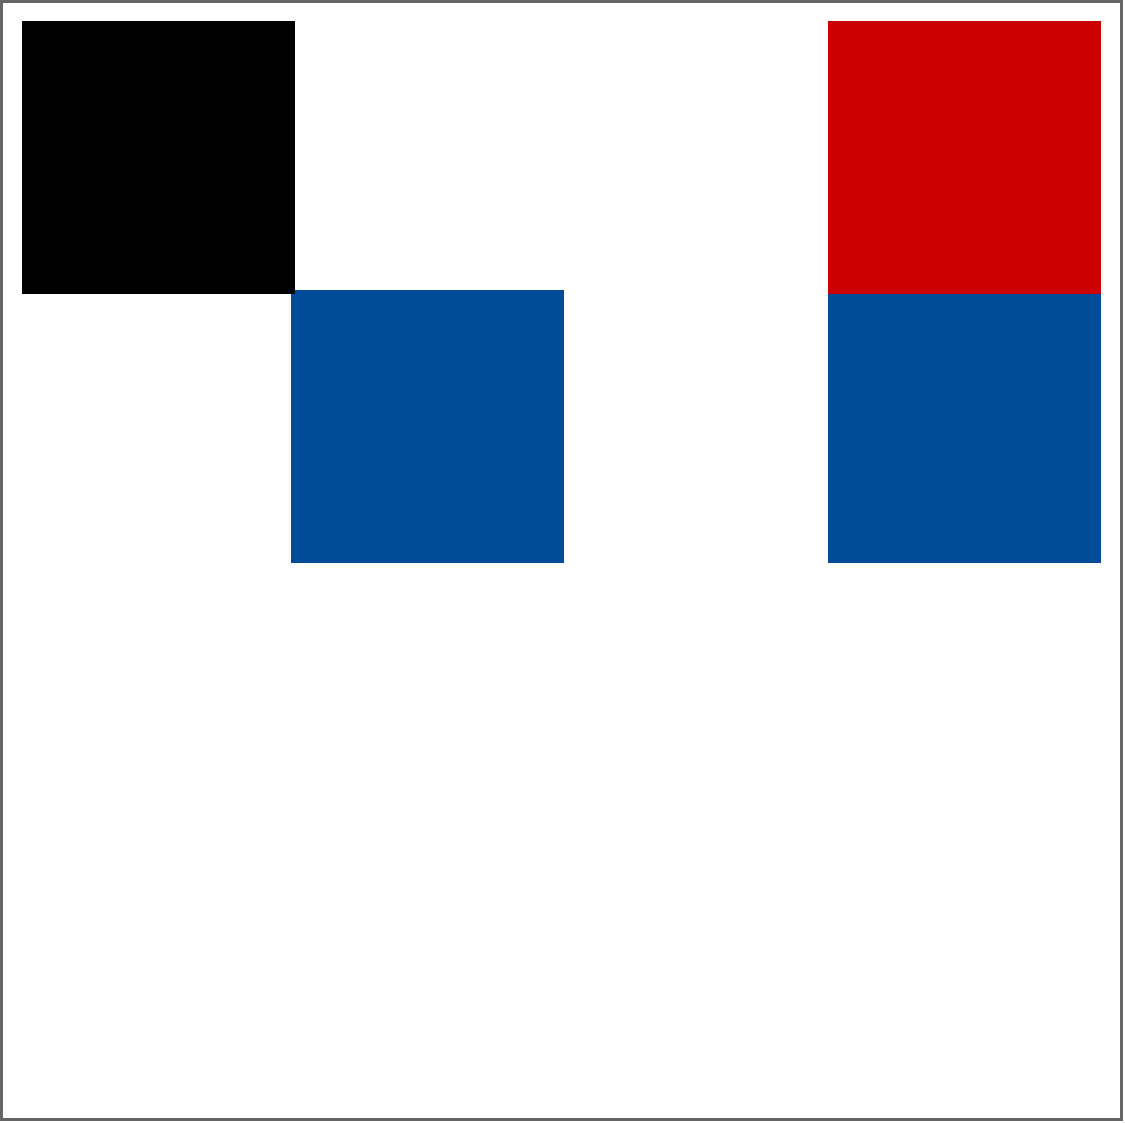
\includegraphics[width=3cm]{state}
\caption{Density matrix in Pauli basis with all components equal
to zero except for $r_{0,0}$, $r_{1,1}$, $r_{1,3}$, and $r_{0,3}$.}
\end{subfigure}
\end{figure}
% }}}

\subsection*{Hypothesis} % {{{
Let us denote $\PCE{n}$ the set of all PCE quantum channels for 
$n$ qubits.
\begin{conj}{}
There exists a set $\Gamma_n\subset\PCE{n}$ that is sufficient (and 
necessary?) to generate the rest of elements in $\PCE{n}$ as 
concatenations of different elements in $\Gamma_n$.
\end{conj}

Let us consider $\E_j\in\Gamma_n$ $(j=1,\ldots,4^{n}-1)$,
and $\Lambda\in\PCE{n}$. All $\Lambda$ are a composition of 
$\E_j$,
\begin{equation}\label{eq:PCE-characterization}
\underbrace{\E_{j_{2n}}\ldots\E_{j_1}}_{k\text{ elements}}=\Lambda,
\hspace{20pt}
j_l\neq j_{l+1},
\hspace{20pt}
k=1,\ldots,2n.
\end{equation}
% }}}
\subsection*{A way to find $\Gamma$} % {{{
PCE quantum channels in $\Gamma_n$ may be found as the quantum 
channels defined by the the coefficients $a_j^{\mu}$ of the $\tau_i$
in the eigenvalues expression of Choi matrix, with $a^{k}_{k}=0$ 
(instead of -1). Let us show the 2-qubits case as an example to illustrate this. 
The eigenvalues of Choi matrix of 2-qubits Pauli Channel are
\begin{align}
\lambda_{1}&=
 \tau _{0,0}+\tau _{0,1}-\tau _{0,2}-\tau _{0,3}+\tau _{1,0}+\tau _{1,1}-\tau _{1,2}-\tau
   _{1,3}-\tau _{2,0}-\tau _{2,1}+\tau _{2,2}+\tau _{2,3}-\tau _{3,0}-\tau _{3,1}+\tau
   _{3,2}+\tau _{3,3} \nonumber \\
\lambda_{2}&=   
 \tau _{0,0}-\tau _{0,1}-\tau _{0,2}+\tau _{0,3}+\tau _{1,0}-\tau _{1,1}-\tau _{1,2}+\tau
   _{1,3}-\tau _{2,0}+\tau _{2,1}+\tau _{2,2}-\tau _{2,3}-\tau _{3,0}+\tau _{3,1}+\tau
   _{3,2}-\tau _{3,3} \nonumber \\
\lambda_{3}&=
 \tau _{0,0}-\tau _{0,1}+\tau _{0,2}-\tau _{0,3}+\tau _{1,0}-\tau _{1,1}+\tau _{1,2}-\tau
   _{1,3}-\tau _{2,0}+\tau _{2,1}-\tau _{2,2}+\tau _{2,3}-\tau _{3,0}+\tau _{3,1}-\tau
   _{3,2}+\tau _{3,3} \nonumber \\
\lambda_{4}&=
 \tau _{0,0}+\tau _{0,1}+\tau _{0,2}+\tau _{0,3}+\tau _{1,0}+\tau _{1,1}+\tau _{1,2}+\tau
   _{1,3}-\tau _{2,0}-\tau _{2,1}-\tau _{2,2}-\tau _{2,3}-\tau _{3,0}-\tau _{3,1}-\tau
   _{3,2}-\tau _{3,3}\nonumber \\
\lambda_{5}&=
 \tau _{0,0}+\tau _{0,1}-\tau _{0,2}-\tau _{0,3}-\tau _{1,0}-\tau _{1,1}+\tau _{1,2}+\tau
   _{1,3}-\tau _{2,0}-\tau _{2,1}+\tau _{2,2}+\tau _{2,3}+\tau _{3,0}+\tau _{3,1}-\tau
   _{3,2}-\tau _{3,3}\nonumber \\
\lambda_{6}&=
 \tau _{0,0}-\tau _{0,1}-\tau _{0,2}+\tau _{0,3}-\tau _{1,0}+\tau _{1,1}+\tau _{1,2}-\tau
   _{1,3}-\tau _{2,0}+\tau _{2,1}+\tau _{2,2}-\tau _{2,3}+\tau _{3,0}-\tau _{3,1}-\tau
   _{3,2}+\tau _{3,3}\nonumber \\
\lambda_{7}&=
 \tau _{0,0}-\tau _{0,1}+\tau _{0,2}-\tau _{0,3}-\tau _{1,0}+\tau _{1,1}-\tau _{1,2}+\tau
   _{1,3}-\tau _{2,0}+\tau _{2,1}-\tau _{2,2}+\tau _{2,3}+\tau _{3,0}-\tau _{3,1}+\tau
   _{3,2}-\tau _{3,3}\nonumber \\
\lambda_{8}&=   
 \tau _{0,0}+\tau _{0,1}+\tau _{0,2}+\tau _{0,3}-\tau _{1,0}-\tau _{1,1}-\tau _{1,2}-\tau
   _{1,3}-\tau _{2,0}-\tau _{2,1}-\tau _{2,2}-\tau _{2,3}+\tau _{3,0}+\tau _{3,1}+\tau
   _{3,2}+\tau _{3,3}\nonumber \\
\lambda_{9}&=   
 \tau _{0,0}+\tau _{0,1}-\tau _{0,2}-\tau _{0,3}-\tau _{1,0}-\tau _{1,1}+\tau _{1,2}+\tau
   _{1,3}+\tau _{2,0}+\tau _{2,1}-\tau _{2,2}-\tau _{2,3}-\tau _{3,0}-\tau _{3,1}+\tau
   _{3,2}+\tau _{3,3}\nonumber \\
\lambda_{10}&=   
 \tau _{0,0}-\tau _{0,1}-\tau _{0,2}+\tau _{0,3}-\tau _{1,0}+\tau _{1,1}+\tau _{1,2}-\tau
   _{1,3}+\tau _{2,0}-\tau _{2,1}-\tau _{2,2}+\tau _{2,3}-\tau _{3,0}+\tau _{3,1}+\tau
   _{3,2}-\tau _{3,3}\nonumber \\
\lambda_{11}&=   
 \tau _{0,0}-\tau _{0,1}+\tau _{0,2}-\tau _{0,3}-\tau _{1,0}+\tau _{1,1}-\tau _{1,2}+\tau
   _{1,3}+\tau _{2,0}-\tau _{2,1}+\tau _{2,2}-\tau _{2,3}-\tau _{3,0}+\tau _{3,1}-\tau
   _{3,2}+\tau _{3,3}\nonumber \\
\lambda_{12}&=   
 \tau _{0,0}+\tau _{0,1}+\tau _{0,2}+\tau _{0,3}-\tau _{1,0}-\tau _{1,1}-\tau _{1,2}-\tau
   _{1,3}+\tau _{2,0}+\tau _{2,1}+\tau _{2,2}+\tau _{2,3}-\tau _{3,0}-\tau _{3,1}-\tau
   _{3,2}-\tau _{3,3}\nonumber \\
\lambda_{13}&=   
 \tau _{0,0}+\tau _{0,1}-\tau _{0,2}-\tau _{0,3}+\tau _{1,0}+\tau _{1,1}-\tau _{1,2}-\tau
   _{1,3}+\tau _{2,0}+\tau _{2,1}-\tau _{2,2}-\tau _{2,3}+\tau _{3,0}+\tau _{3,1}-\tau
   _{3,2}-\tau _{3,3}\nonumber \\
\lambda_{14}&=   
 \tau _{0,0}-\tau _{0,1}-\tau _{0,2}+\tau _{0,3}+\tau _{1,0}-\tau _{1,1}-\tau _{1,2}+\tau
   _{1,3}+\tau _{2,0}-\tau _{2,1}-\tau _{2,2}+\tau _{2,3}+\tau _{3,0}-\tau _{3,1}-\tau
   _{3,2}+\tau _{3,3}\nonumber \\
\lambda_{15}&=   
 \tau _{0,0}-\tau _{0,1}+\tau _{0,2}-\tau _{0,3}+\tau _{1,0}-\tau _{1,1}+\tau _{1,2}-\tau
   _{1,3}+\tau _{2,0}-\tau _{2,1}+\tau _{2,2}-\tau _{2,3}+\tau _{3,0}-\tau _{3,1}+\tau
   _{3,2}-\tau _{3,3}\nonumber \\
\lambda_{16}&=  
 \tau _{0,0}+\tau _{0,1}+\tau _{0,2}+\tau _{0,3}+\tau _{1,0}+\tau _{1,1}+\tau _{1,2}+\tau
   _{1,3}+\tau _{2,0}+\tau _{2,1}+\tau _{2,2}+\tau _{2,3}+\tau _{3,0}+\tau _{3,1}+\tau
   _{3,2}+\tau _{3,3}. 
\end{align}

Now, taking all $\tau_{i,j}$ with coefficients $-1$ equal to zero 
one is led to 16 elements of $\PCE{2}$ (one for each eigenvalue): \newline

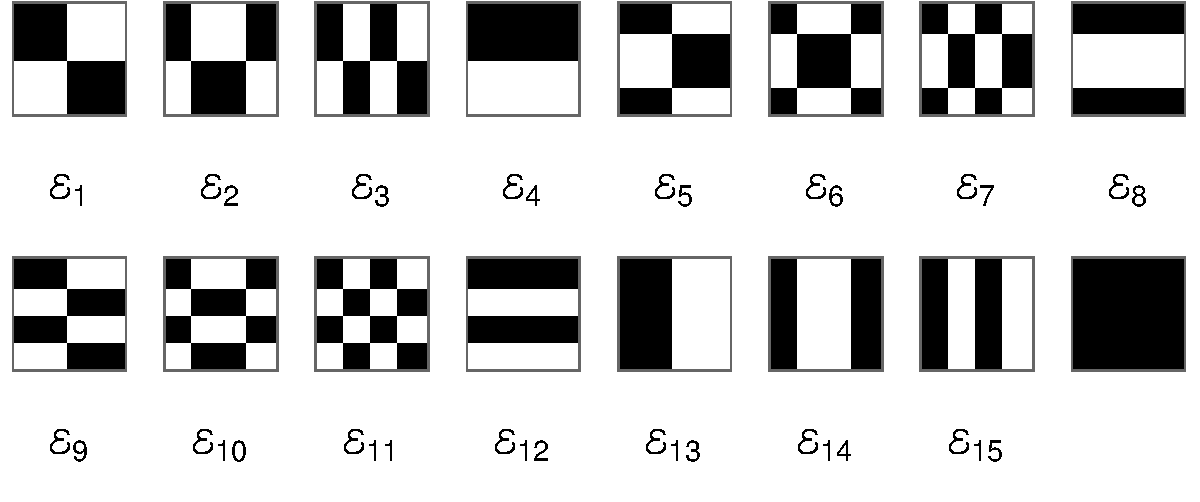
\includegraphics[width=\textwidth]{2Q-fundamentals}

The first 15 elements are the elements of $\Gamma_2$. 

For the sake
of completeness let us show how to construct all elements in $\PCE{2}$
from $\Gamma_2$. Recall that $\PCE{2}$ can be ordered in 
equivalence classes with PCE quantum channels that are 
connected via particle swaps and local permutations 
of basis.

\begin{itemize}
\item \textbf{8 components:} 
\begin{itemize}
\item C$_1^8$: $\E_{13}$\newline
\begin{tabular}{m{2cm} m{2cm} m{2cm}}
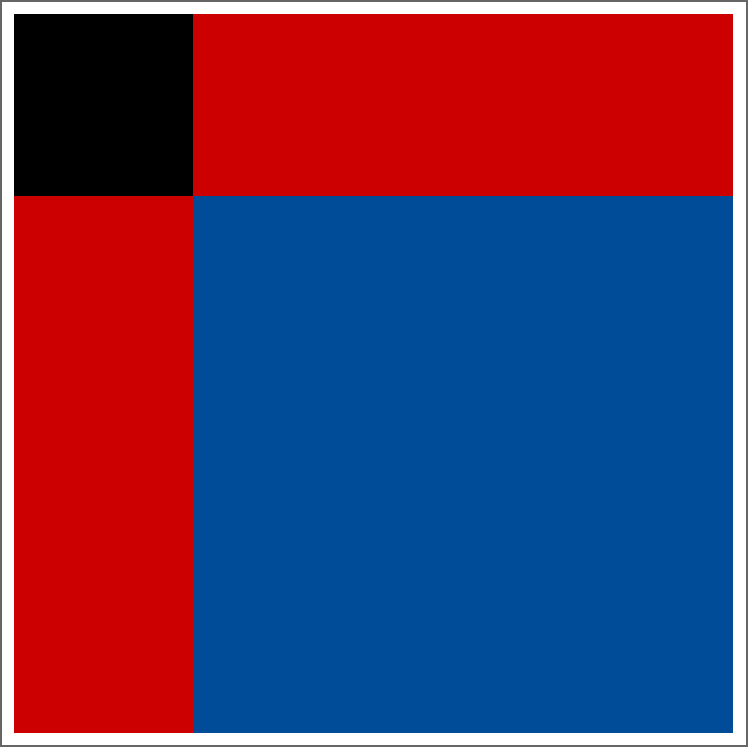
\includegraphics[width=2.2cm]{img-JA/id}  
& \hspace{0.8cm}$\longrightarrow$ 
& 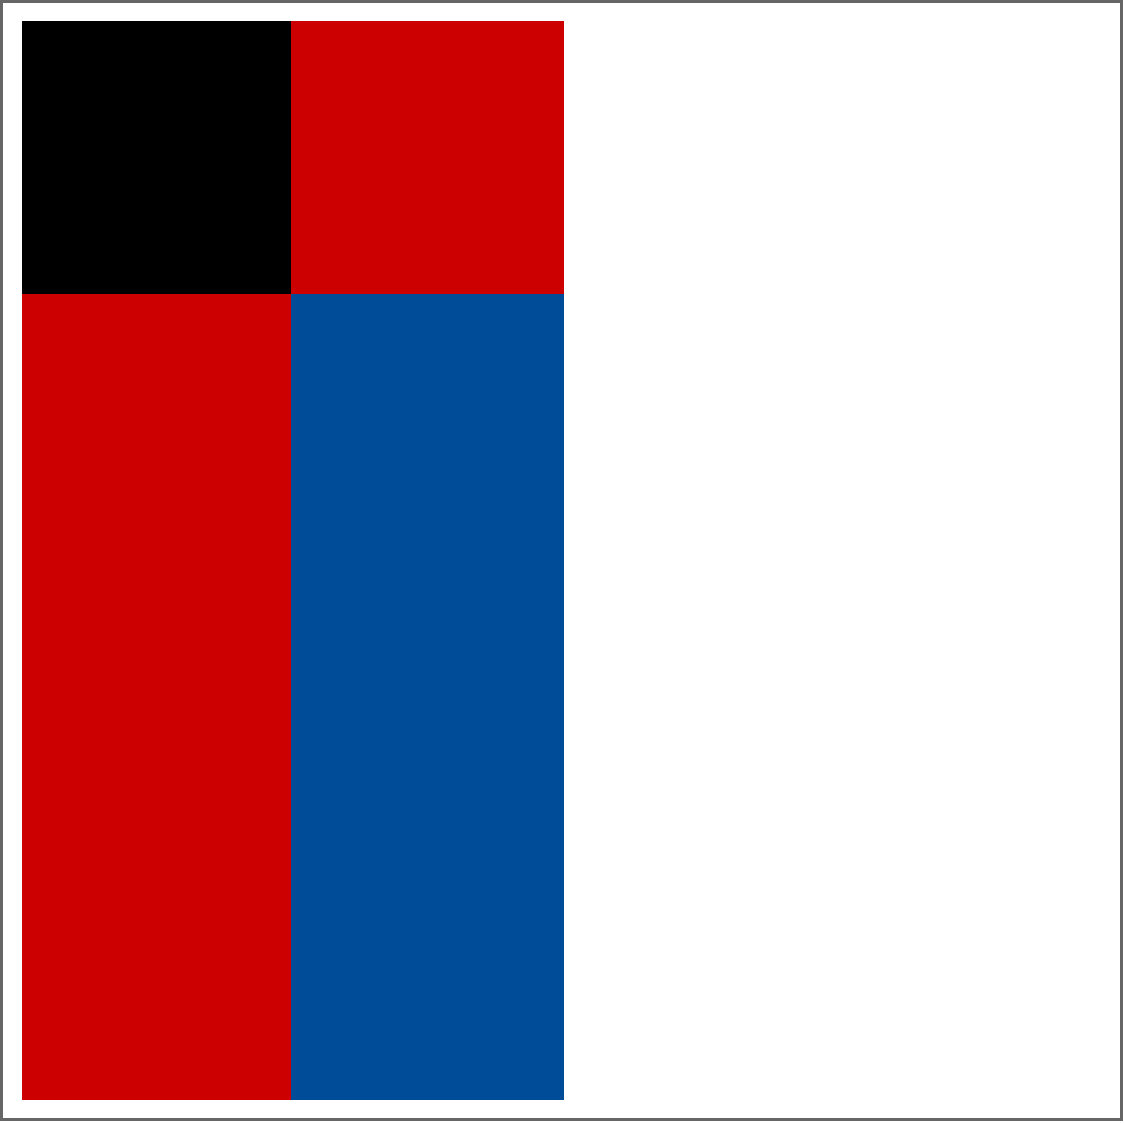
\includegraphics[width=2.2cm]{C81} \\ 
 & 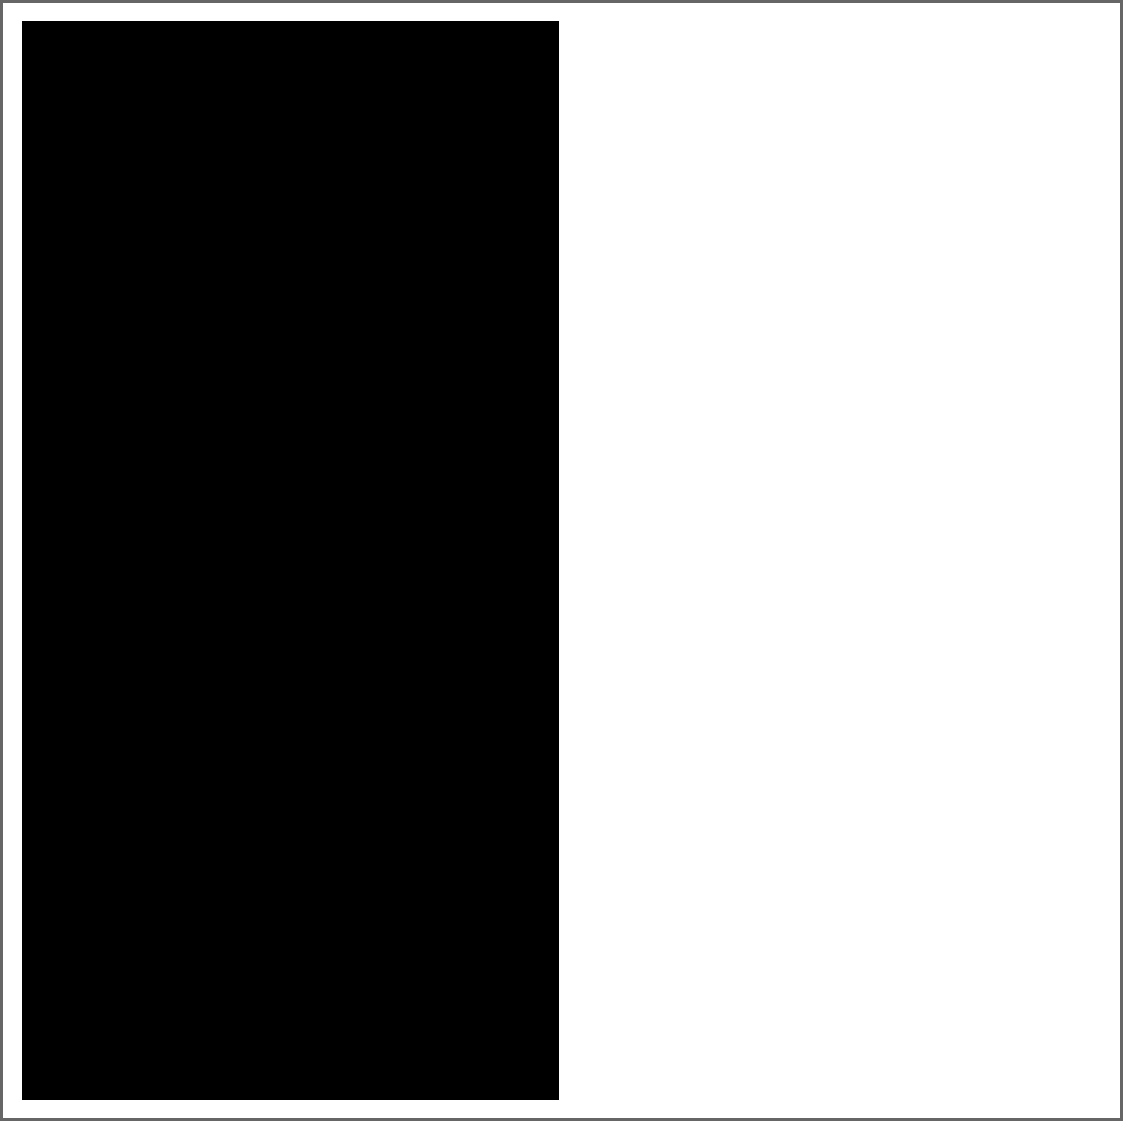
\includegraphics[width=2.2cm]{ruleC81} & 
\end{tabular} 

\item C$_2^8$: $\E_1$\newline
\begin{tabular}{m{2cm} m{2cm} m{2cm}}
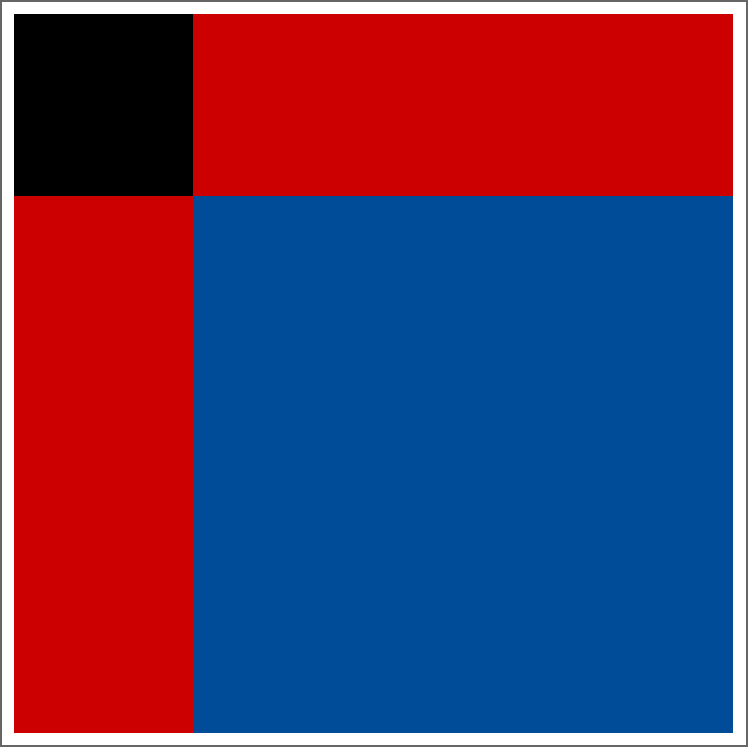
\includegraphics[width=2.2cm]{img-JA/id}  
& \hspace{0.8cm}$\longrightarrow$ 
& 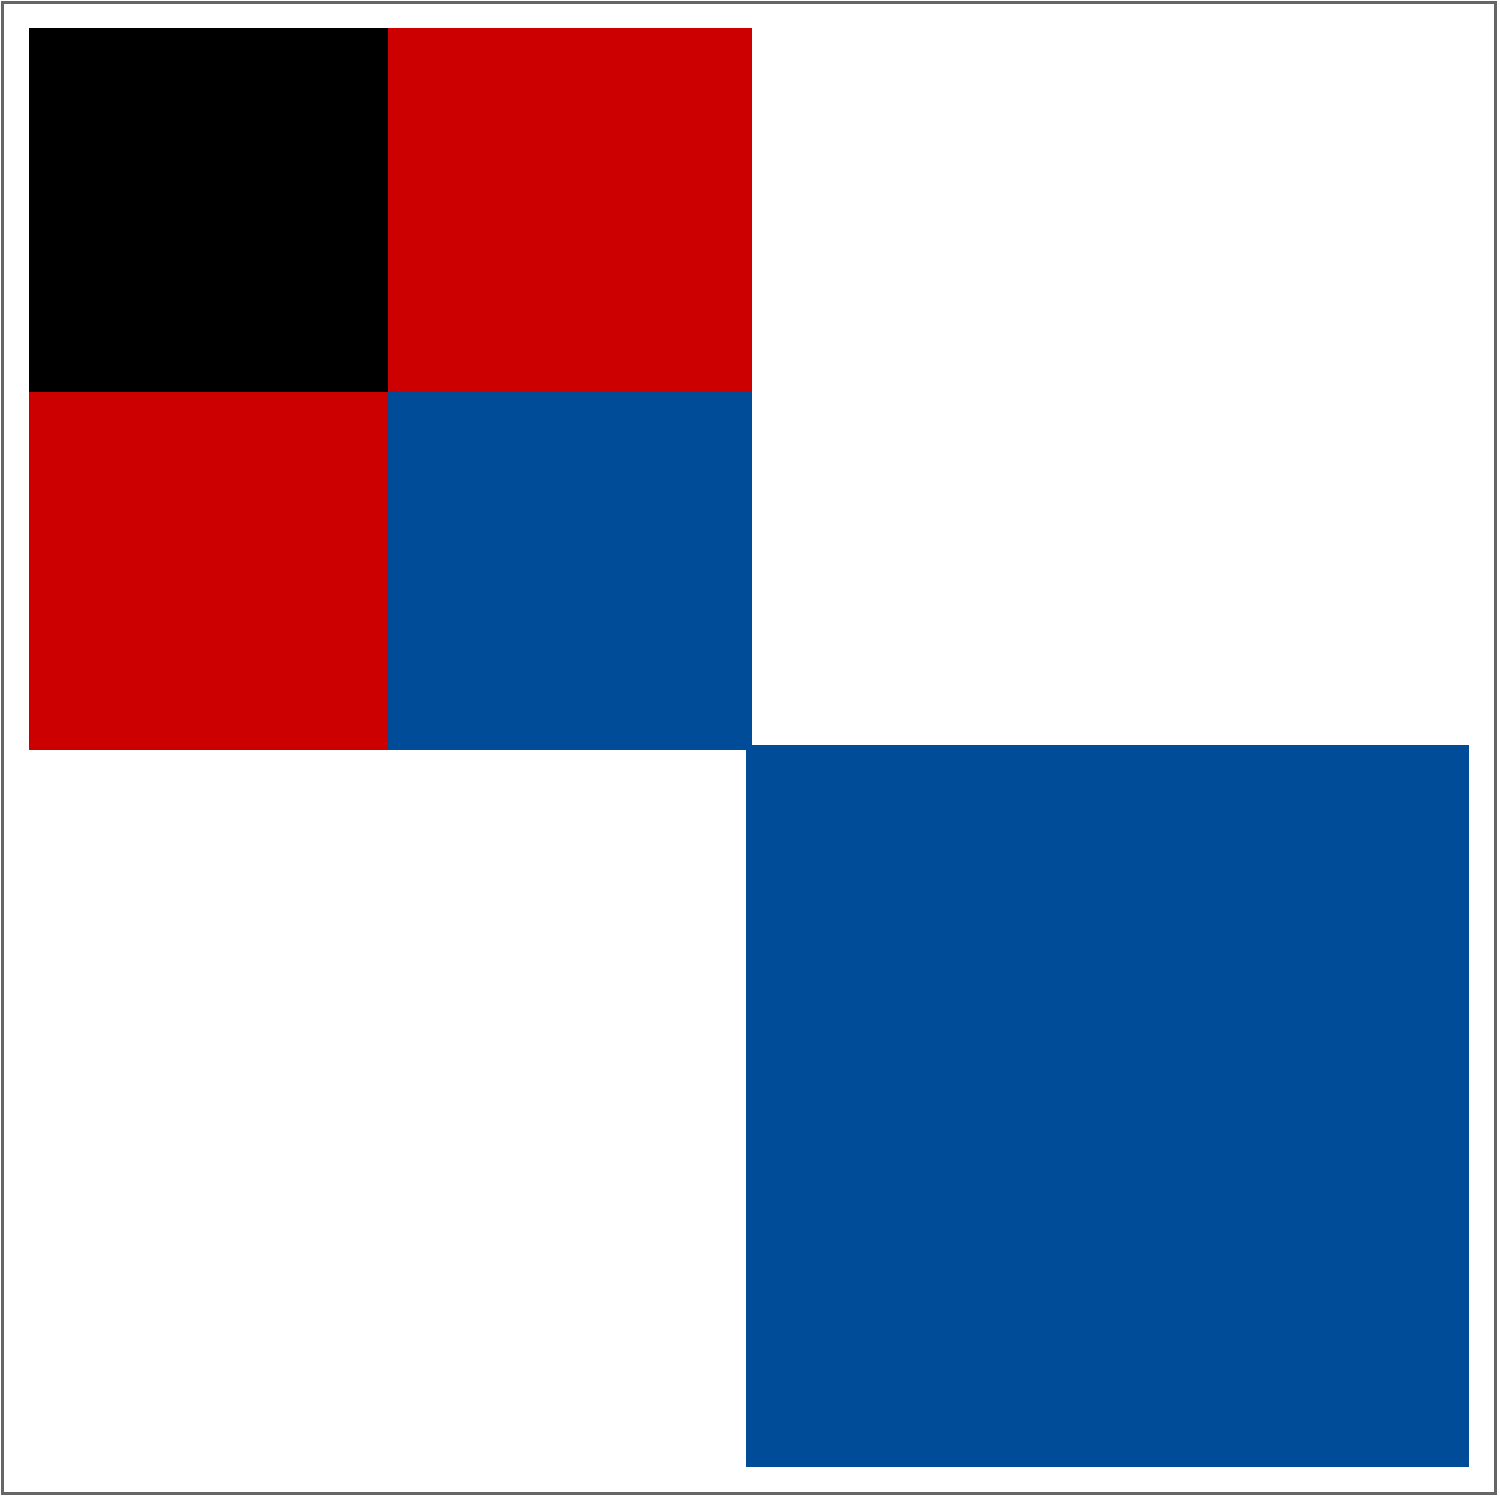
\includegraphics[width=2.2cm]{img-JA/8comp}\\ 
 & 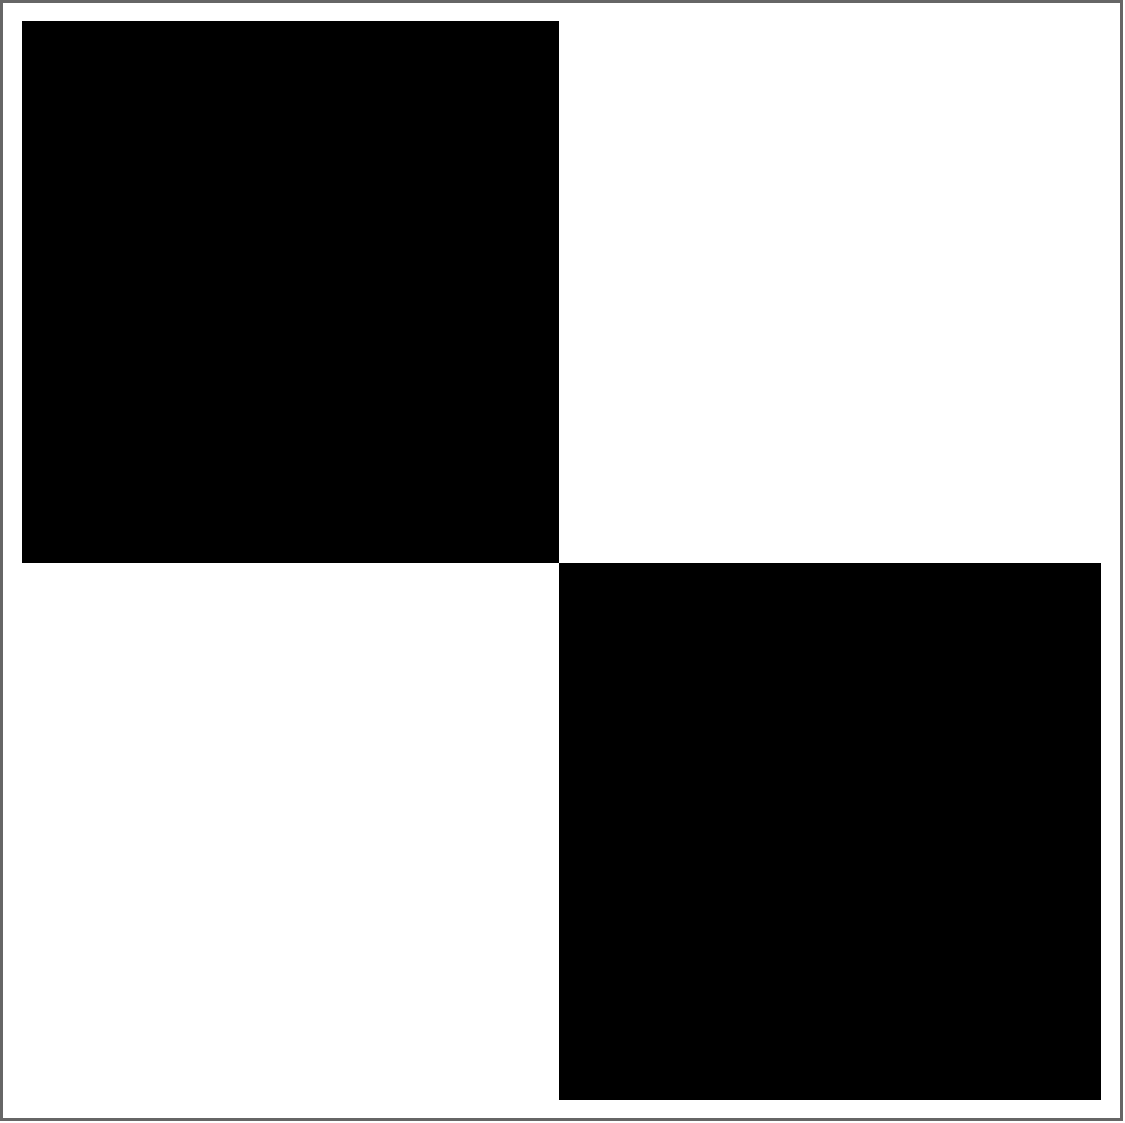
\includegraphics[width=2.2cm]{img-JA/16To8} &  
\end{tabular} 
\end{itemize}

\item \textbf{4 components:} \newline
\begin{itemize}
\item C$_1^4$: $\E_{15}\E_{13}$\newline
\begin{tabular}{m{2cm} m{2cm} m{2cm} m{2cm} m{2cm}}
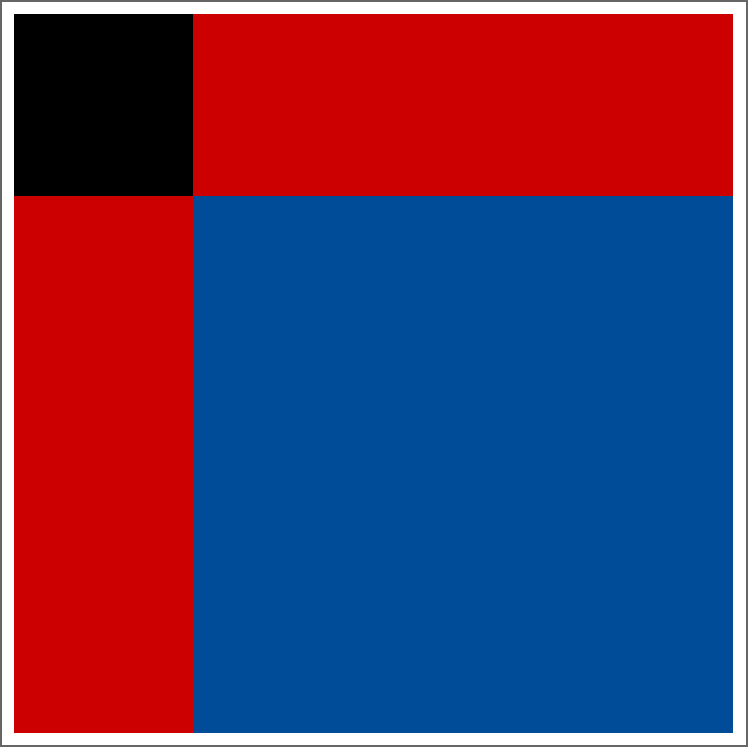
\includegraphics[width=2.2cm]{img-JA/id}  
& \hspace{0.8cm}$\longrightarrow$ 
& 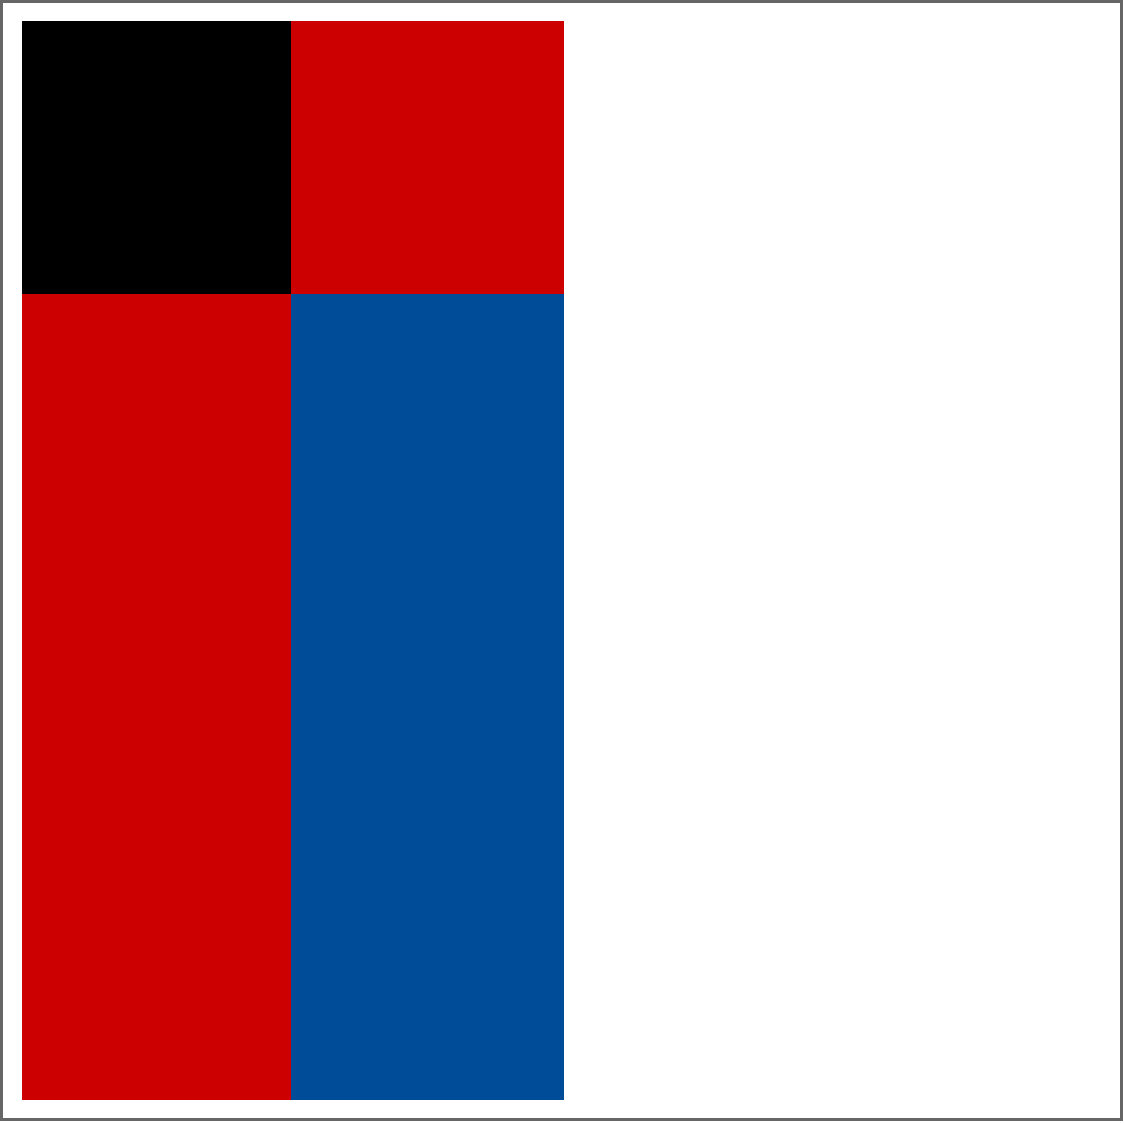
\includegraphics[width=2.2cm]{C81} 
& \hspace{0.8cm}$\longrightarrow$ 
& 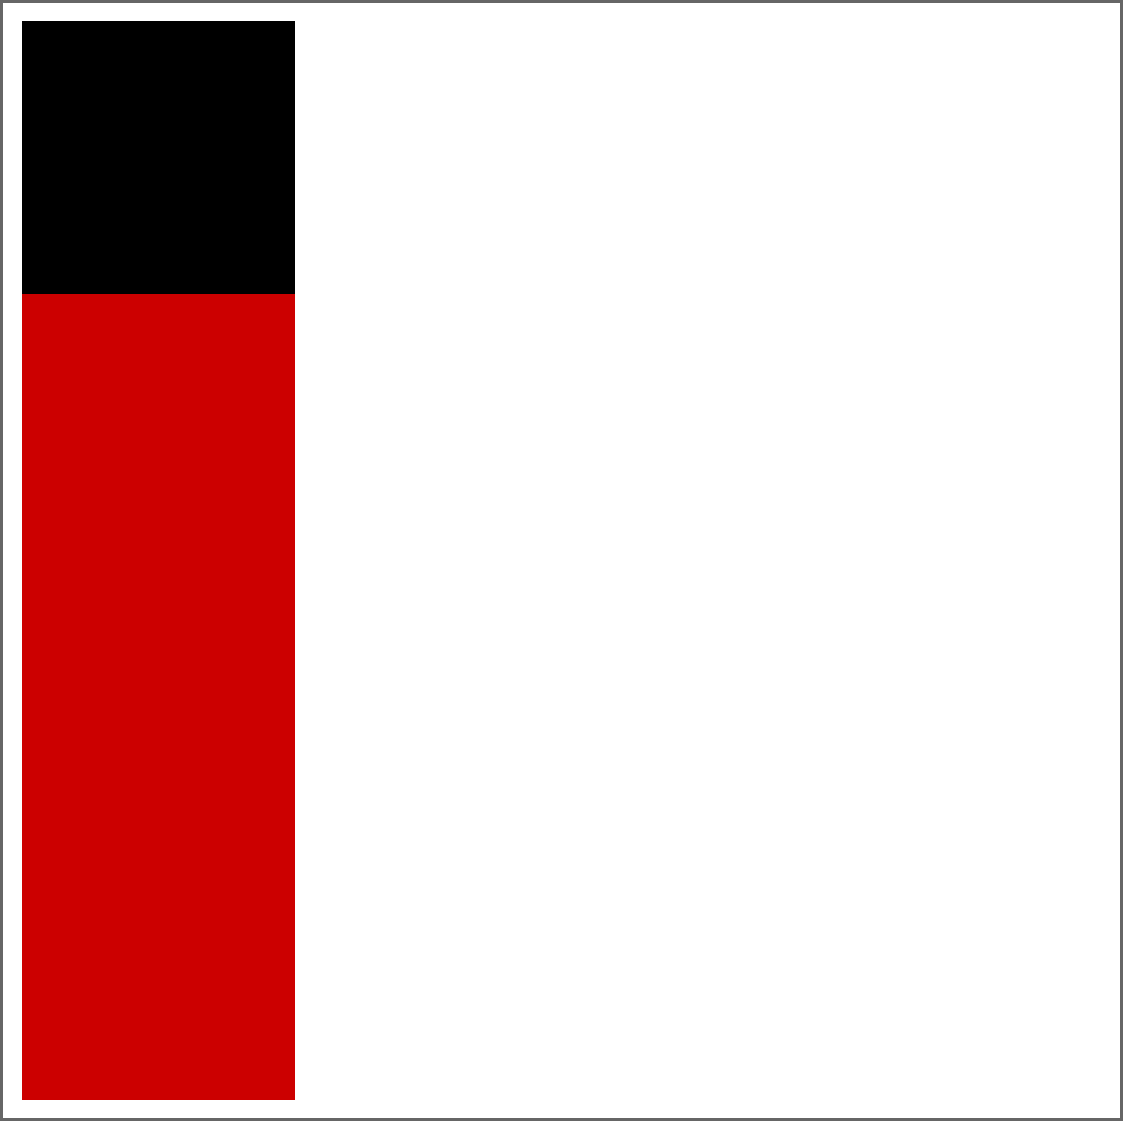
\includegraphics[width=2.2cm]{C41}\\ 
 & 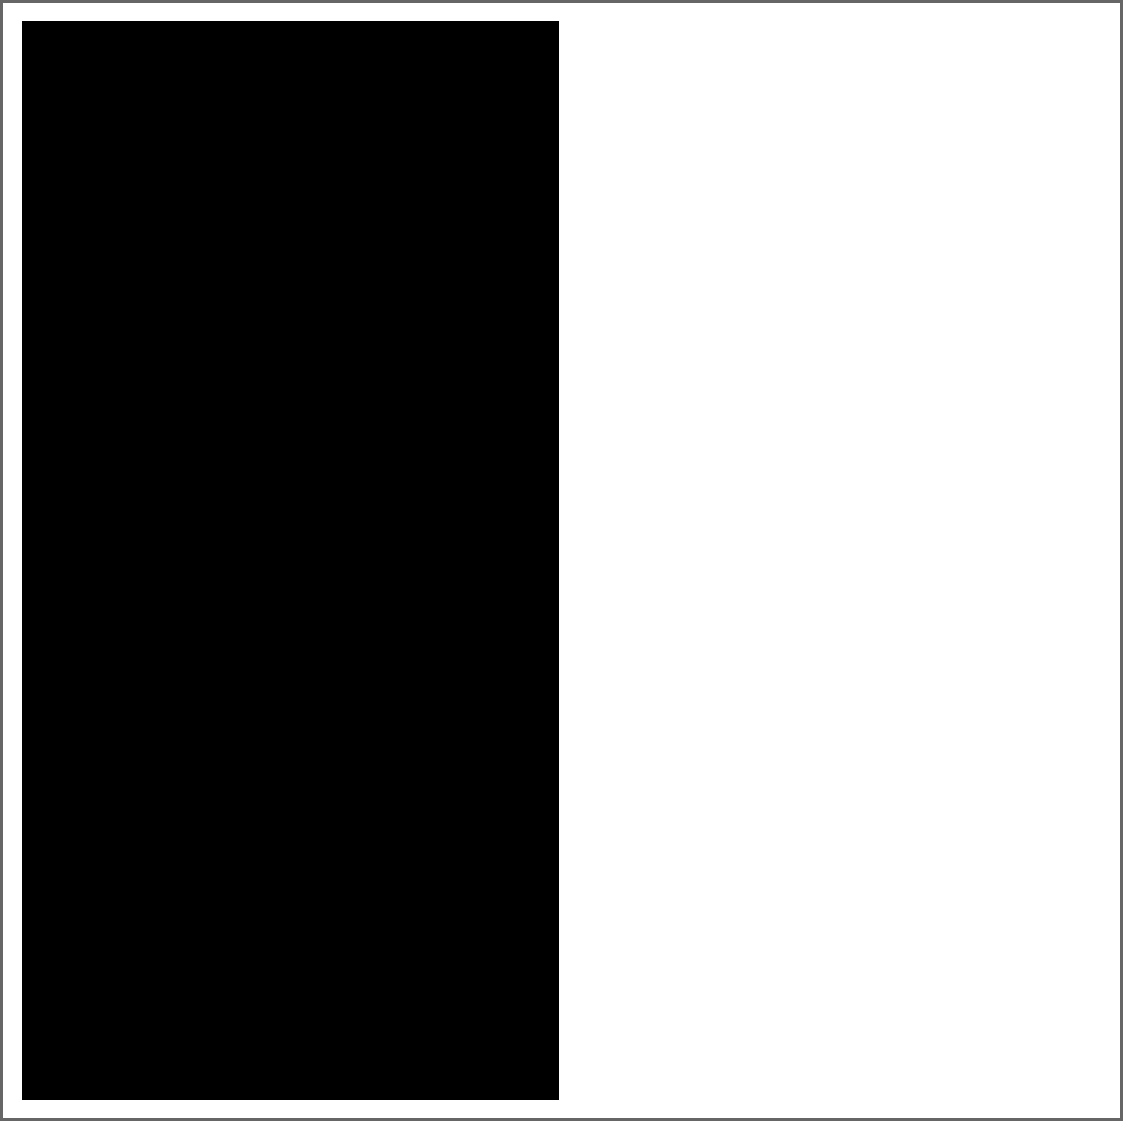
\includegraphics[width=2.2cm]{ruleC81} &  
 & 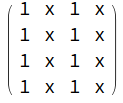
\includegraphics[width=2.2cm]{ruleC81_2} &\\ 
\end{tabular} 

\item C$_2^4$: $\E_{13}\E_1$\newline
\begin{tabular}{m{2cm} m{2cm} m{2cm} m{2cm} m{2cm}}
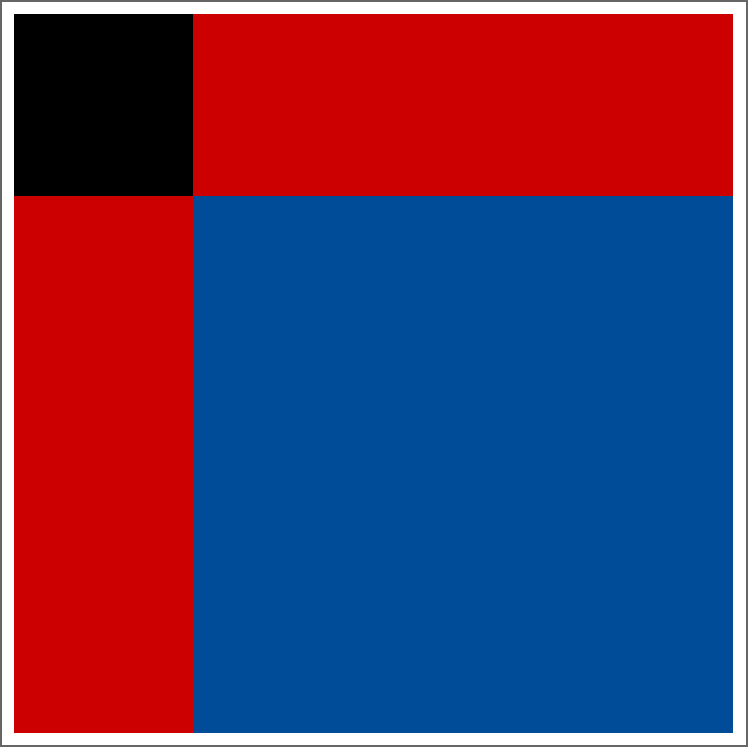
\includegraphics[width=2.2cm]{img-JA/id}  
& \hspace{0.8cm}$\longrightarrow$ 
& 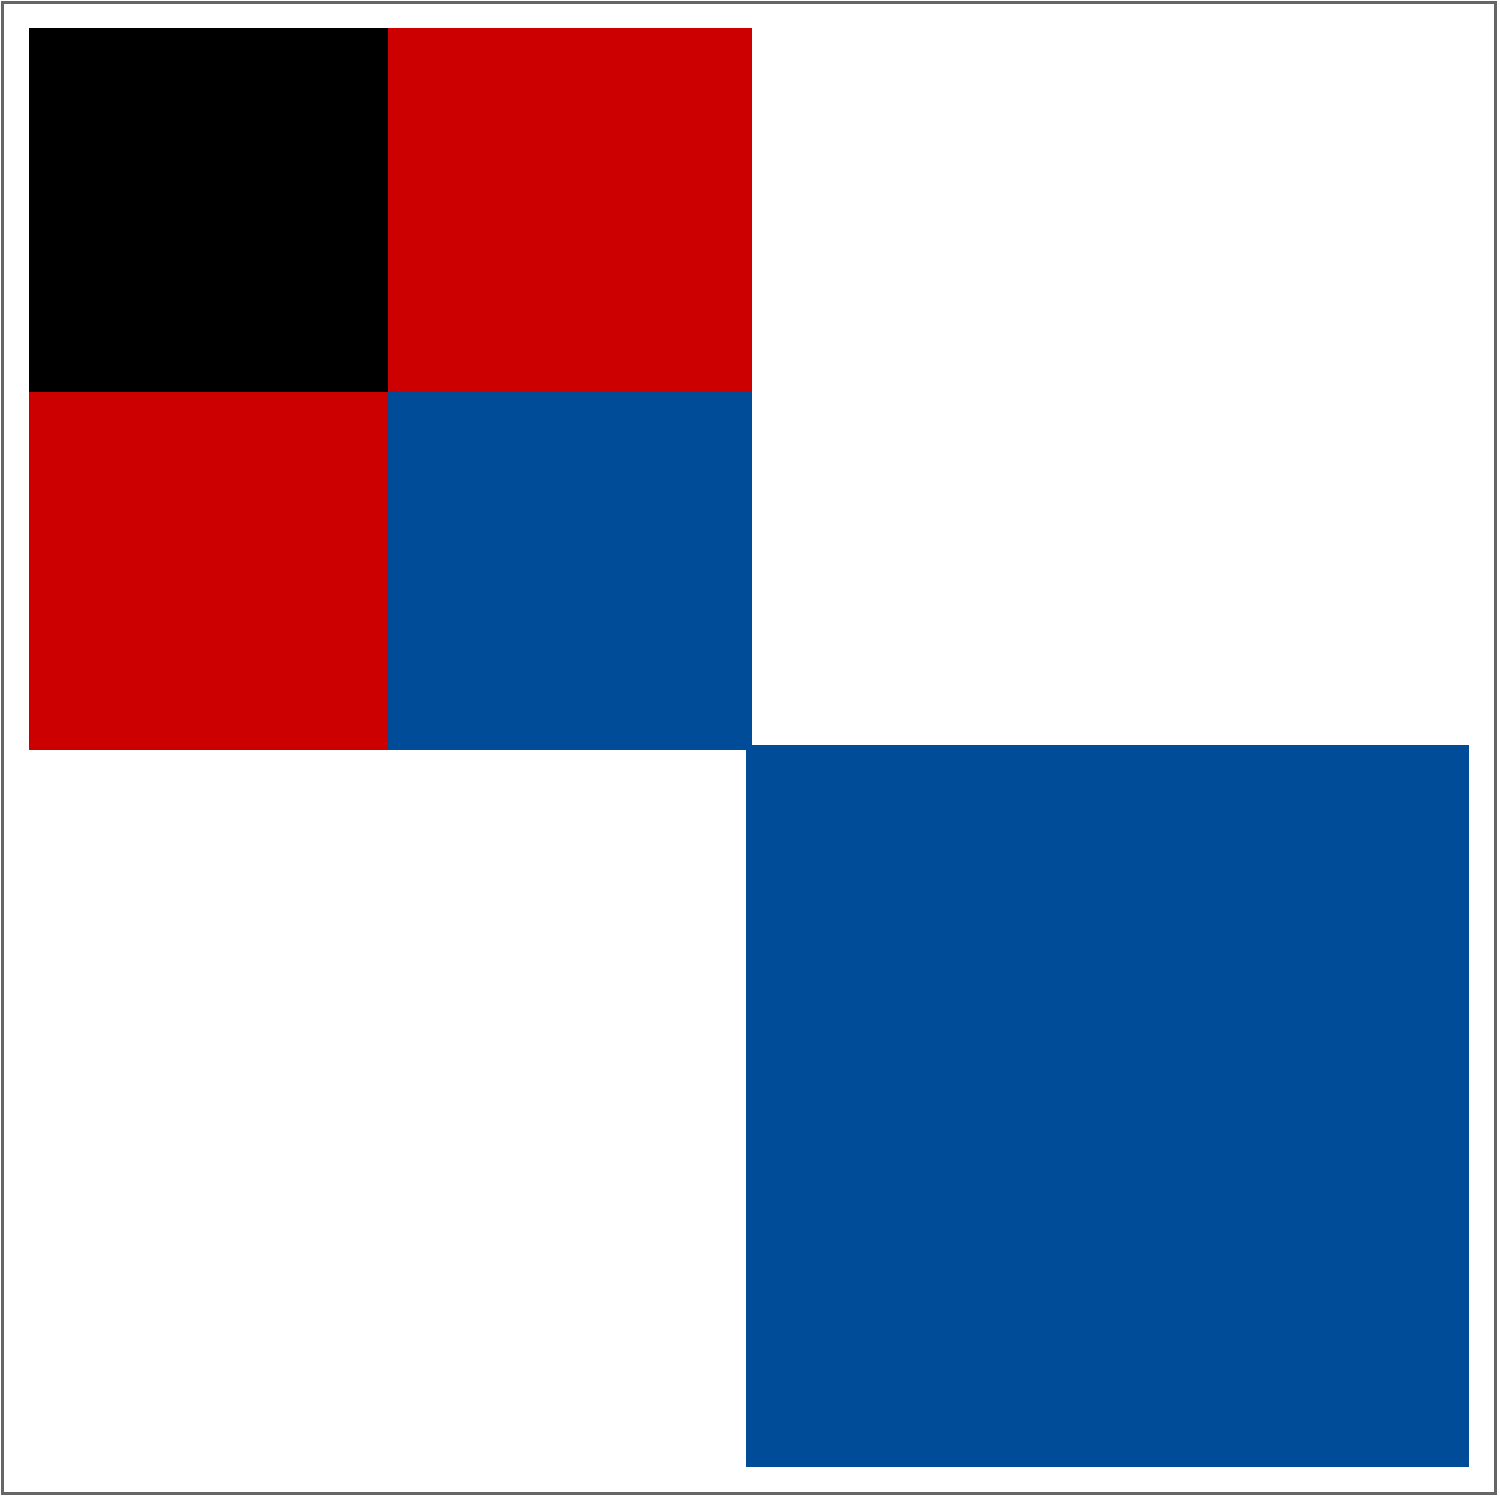
\includegraphics[width=2.2cm]{img-JA/8comp} 
& \hspace{0.8cm}$\longrightarrow$ 
& 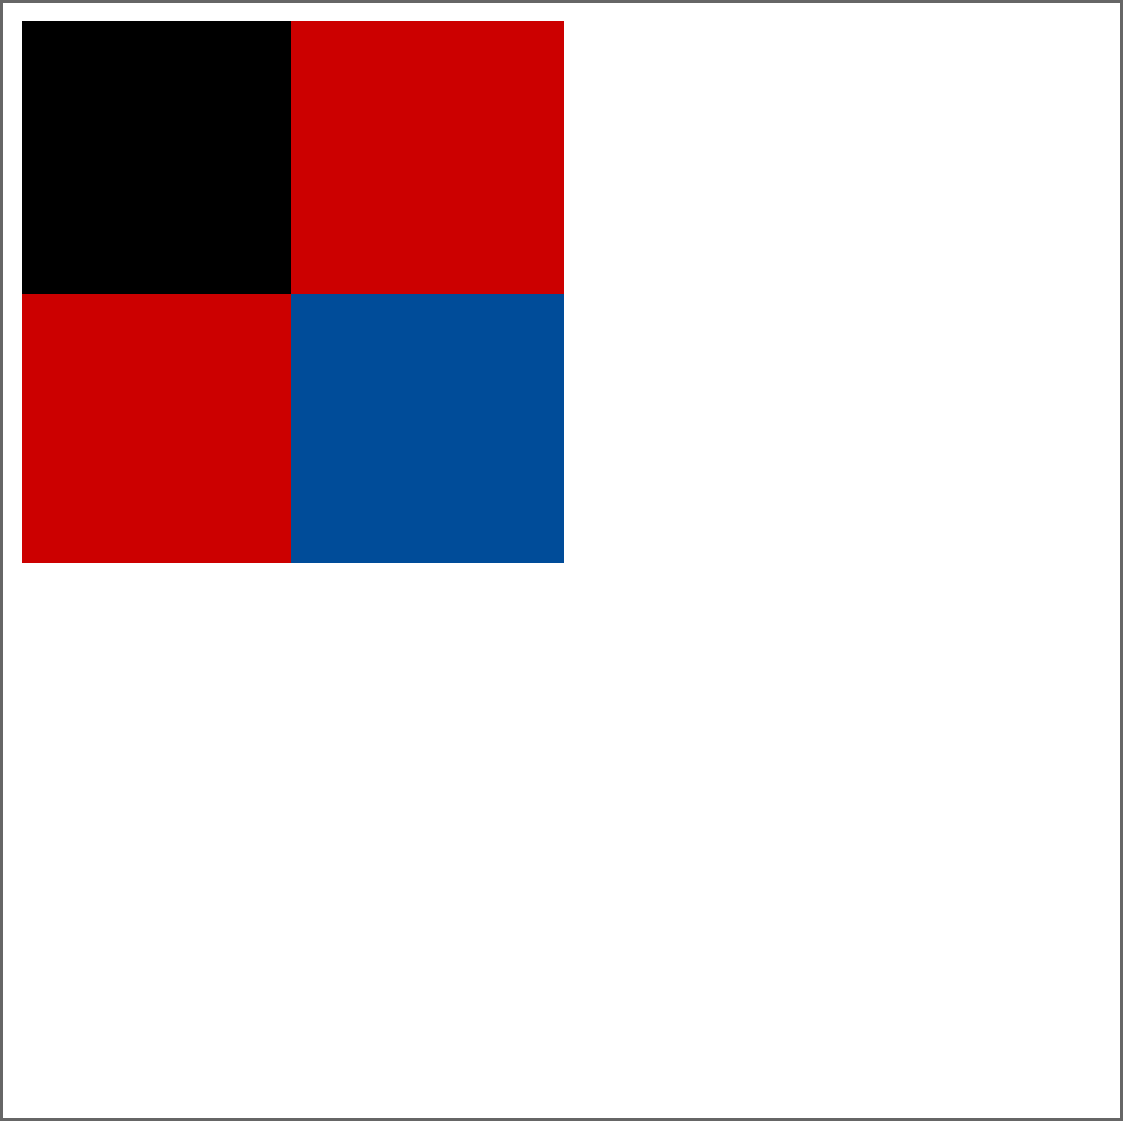
\includegraphics[width=2.2cm]{C42}\\ 
 & 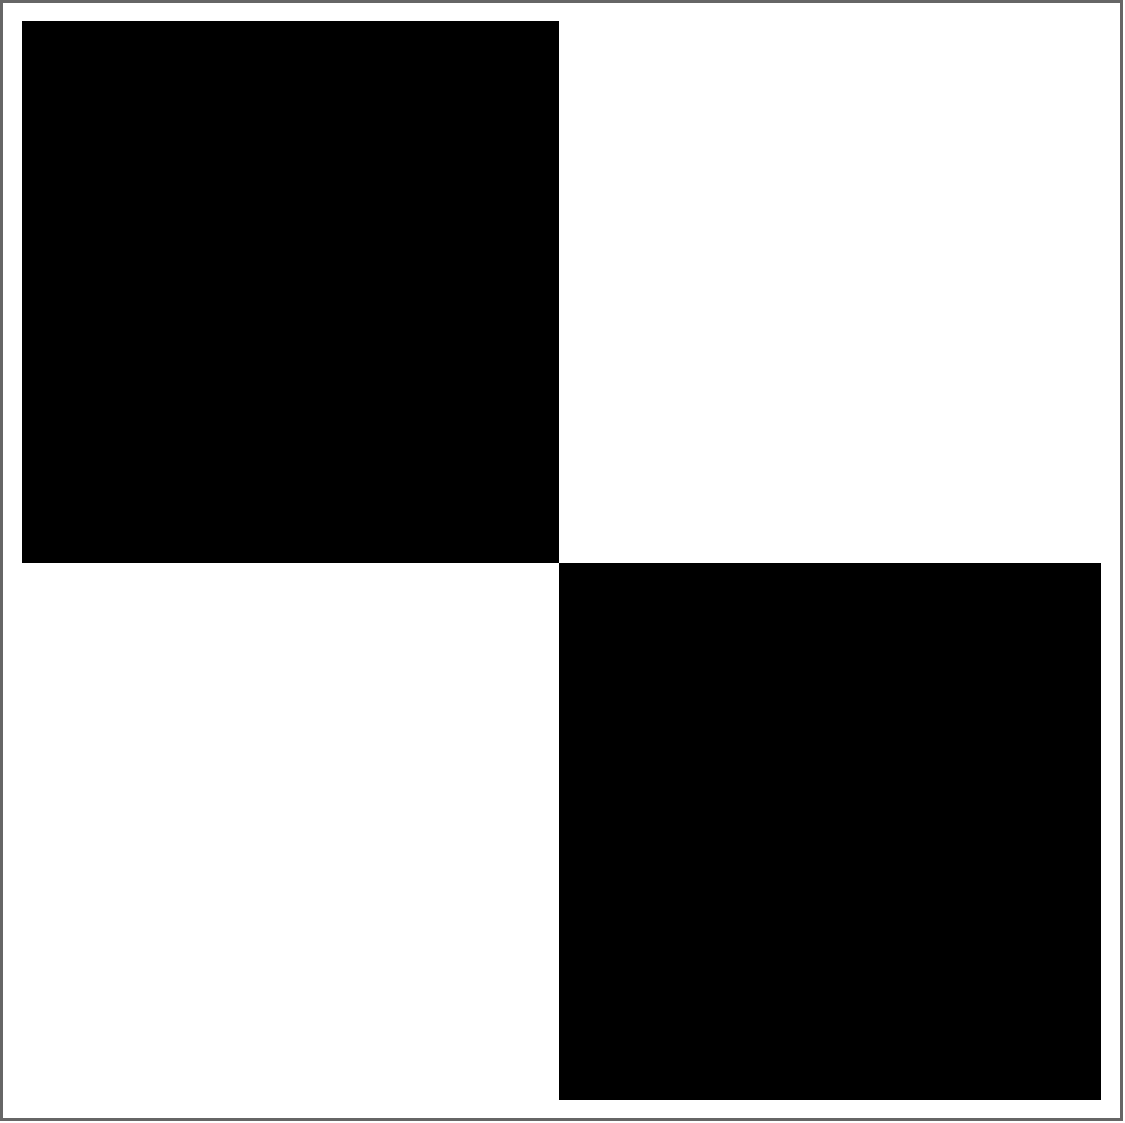
\includegraphics[width=2.2cm]{img-JA/16To8} &  
 & 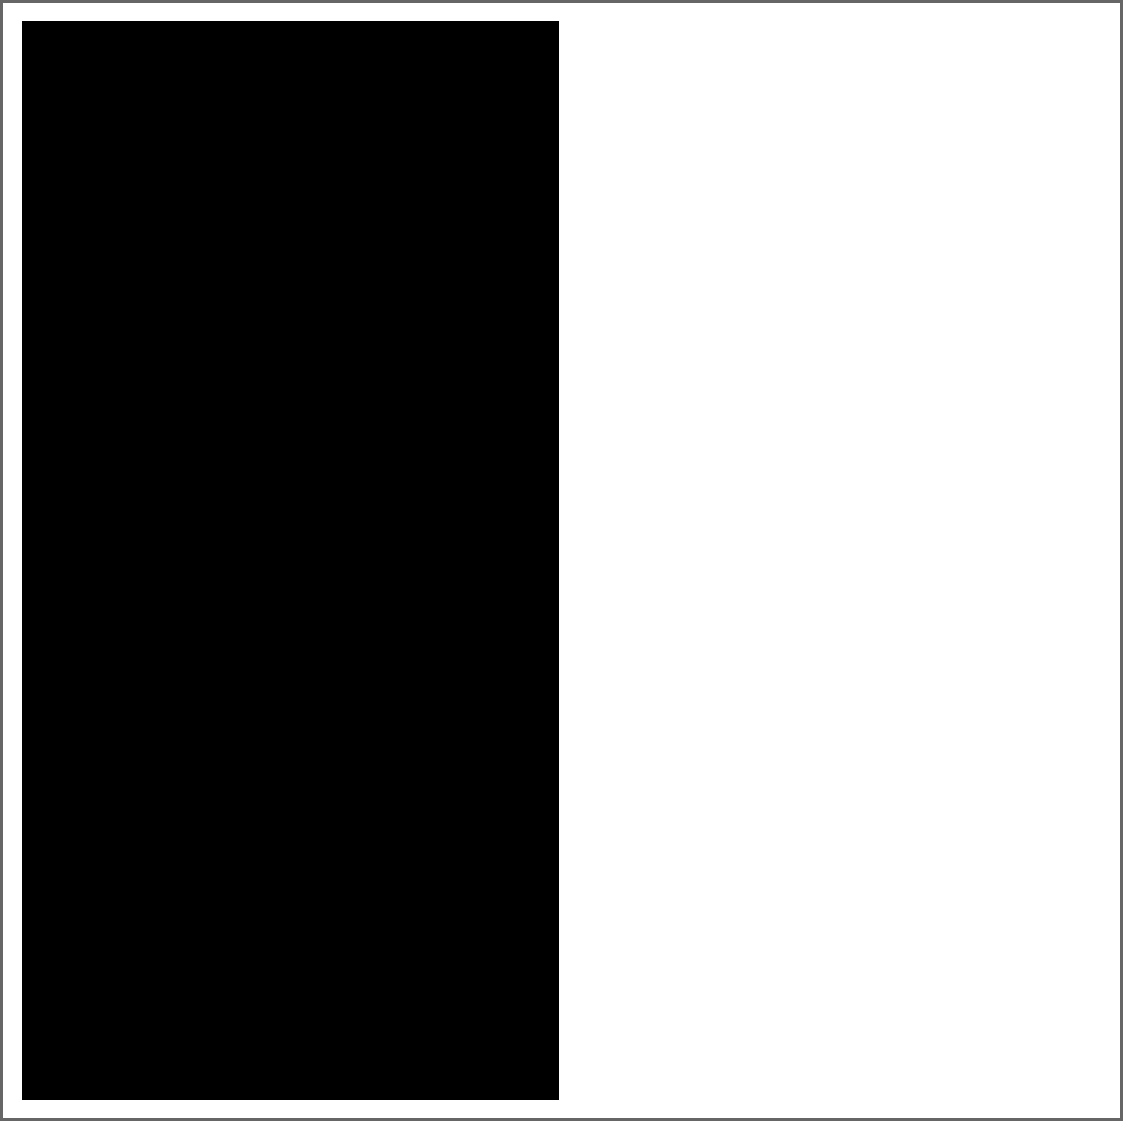
\includegraphics[width=2.2cm]{ruleC81} &\\ 
\end{tabular} 

\pagebreak
\item C$_3^4$: $\E_{15}\E_{1}$\newline
\begin{tabular}{m{2cm} m{2cm} m{2cm} m{2cm} m{2cm}}
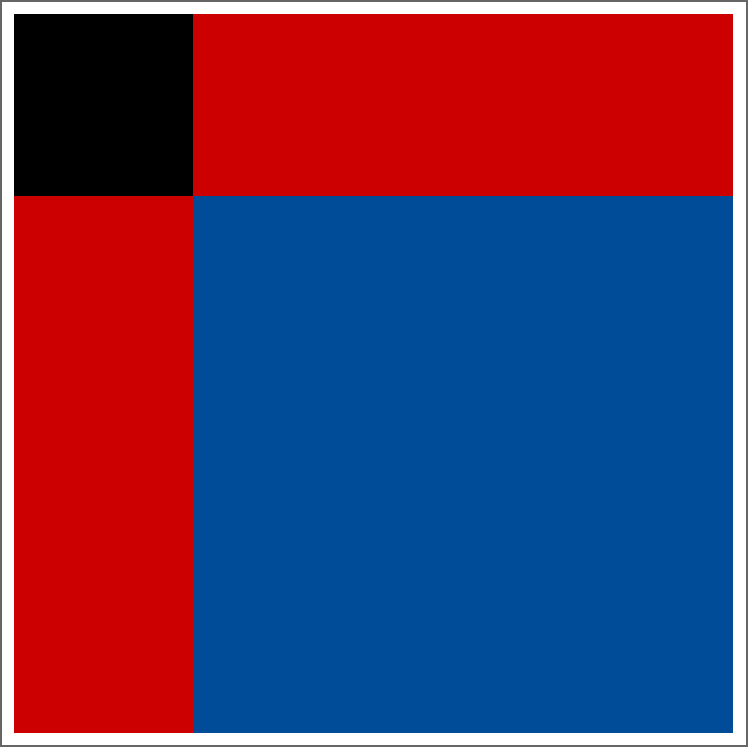
\includegraphics[width=2.2cm]{img-JA/id}  
& \hspace{0.8cm}$\longrightarrow$ 
& 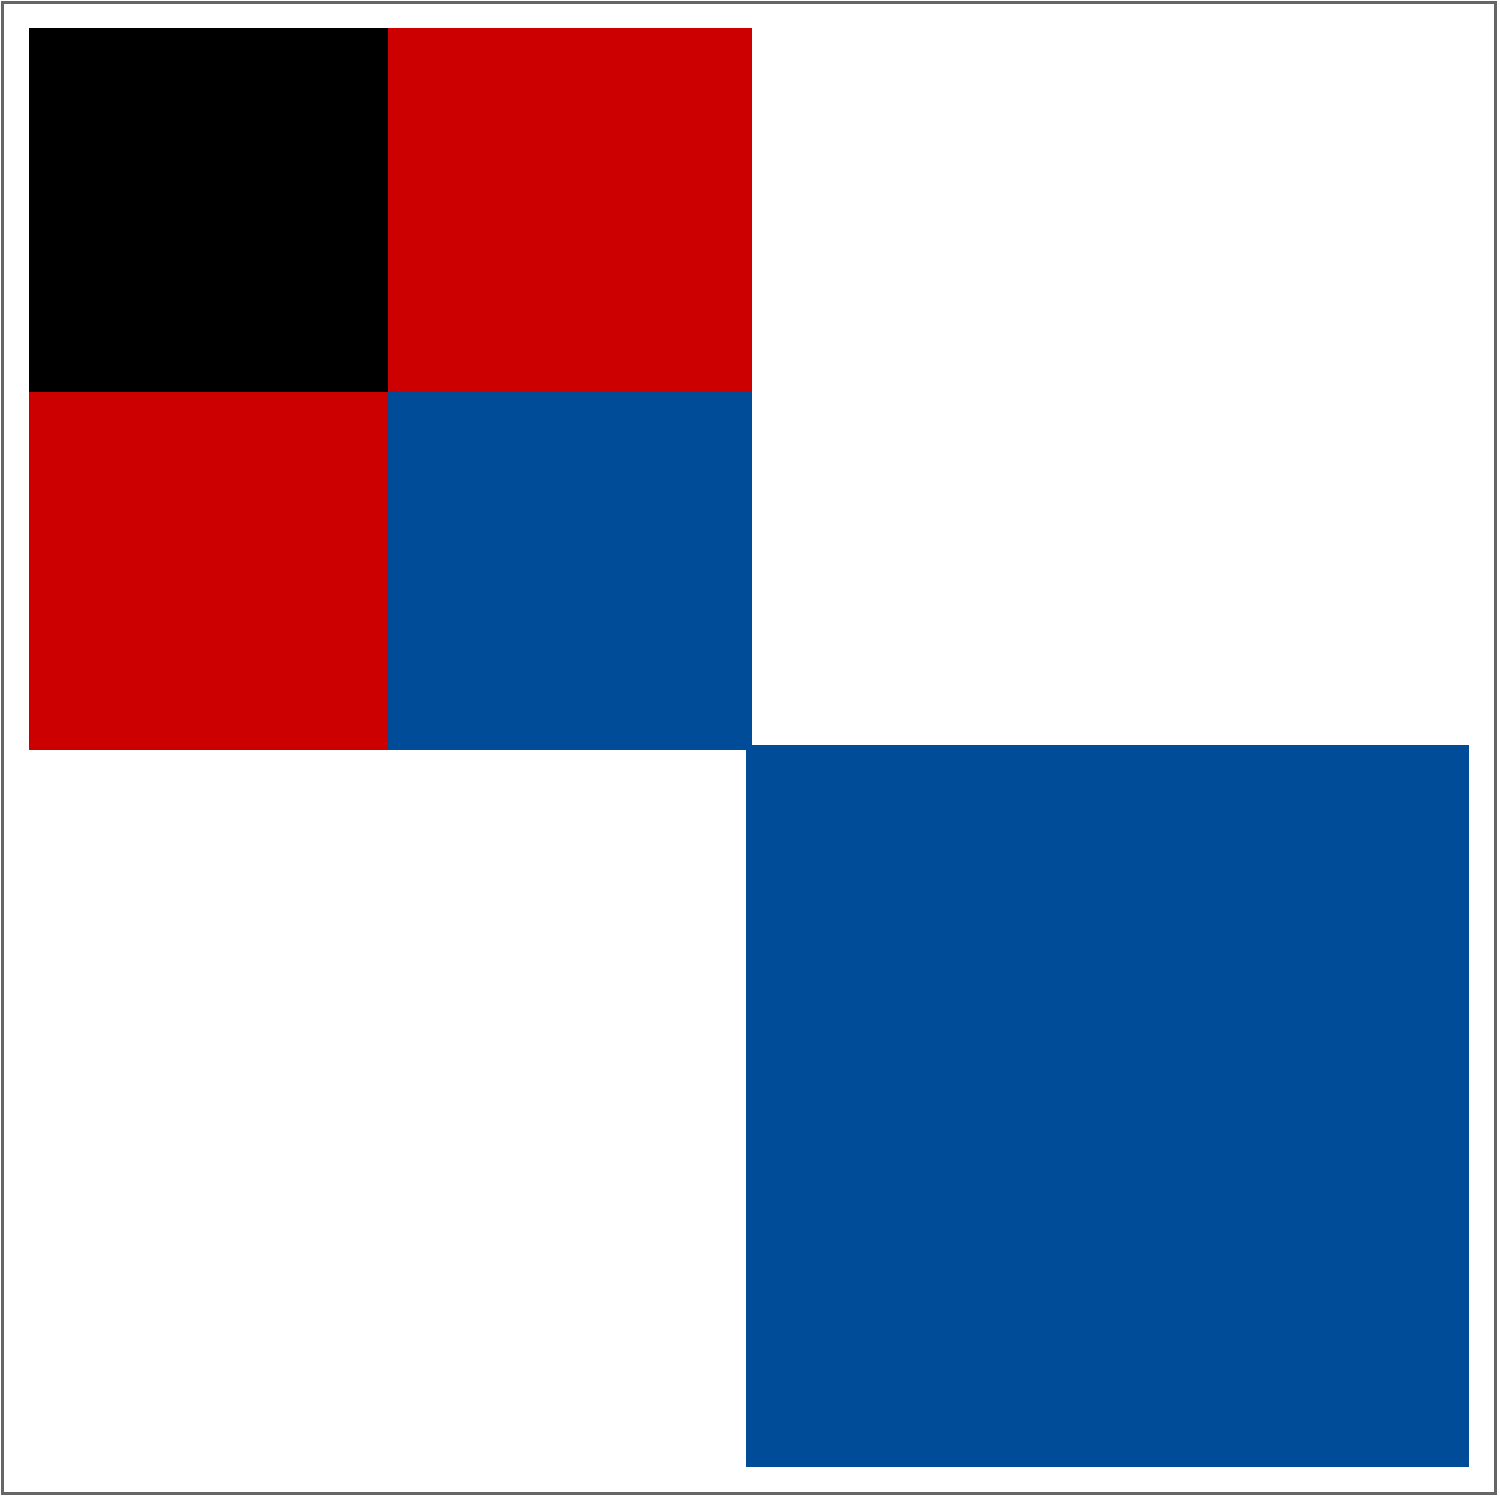
\includegraphics[width=2.2cm]{img-JA/8comp} 
& \hspace{0.8cm}$\longrightarrow$ 
& 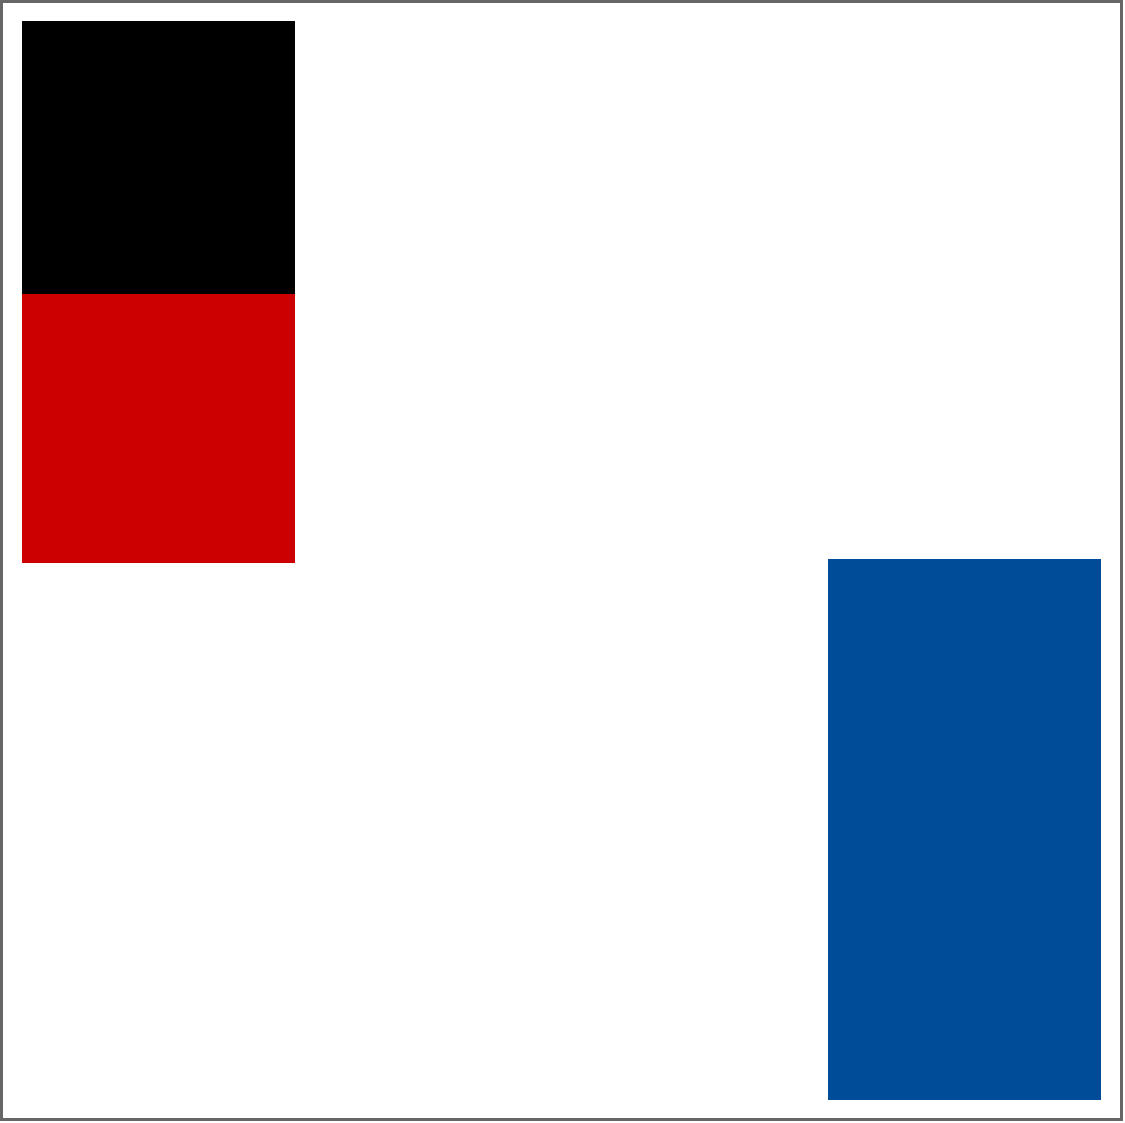
\includegraphics[width=2.2cm]{C43}\\ 
 & 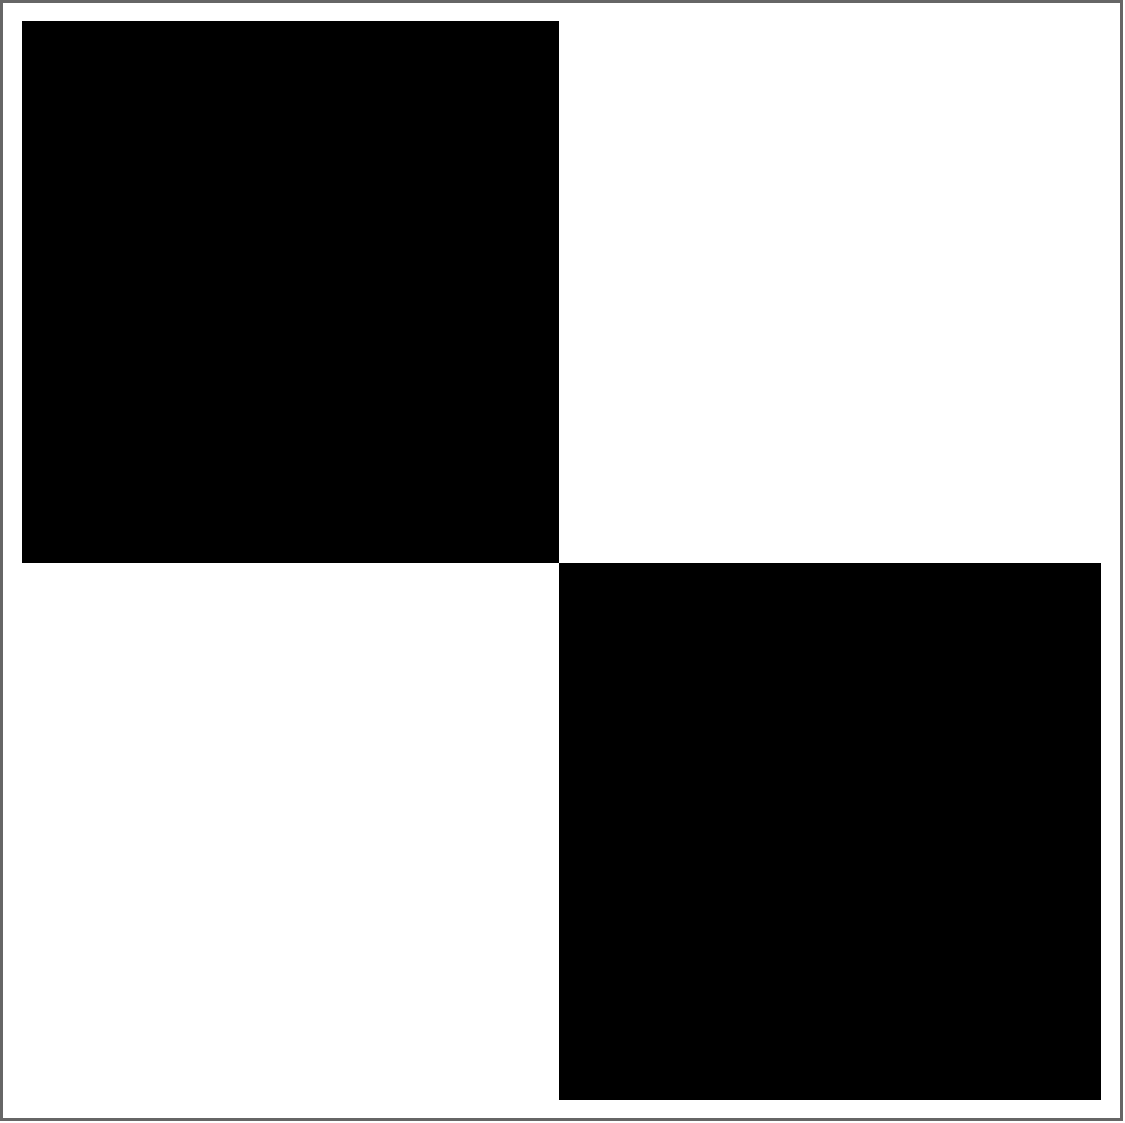
\includegraphics[width=2.2cm]{img-JA/16To8} &  
 & 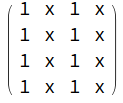
\includegraphics[width=2.2cm]{ruleC81_2} &\\ 
\end{tabular} 

\item C$_4^4$: $\E_7\E_1$\newline
\begin{tabular}{m{2cm} m{2cm} m{2cm} m{2cm} m{2cm}}
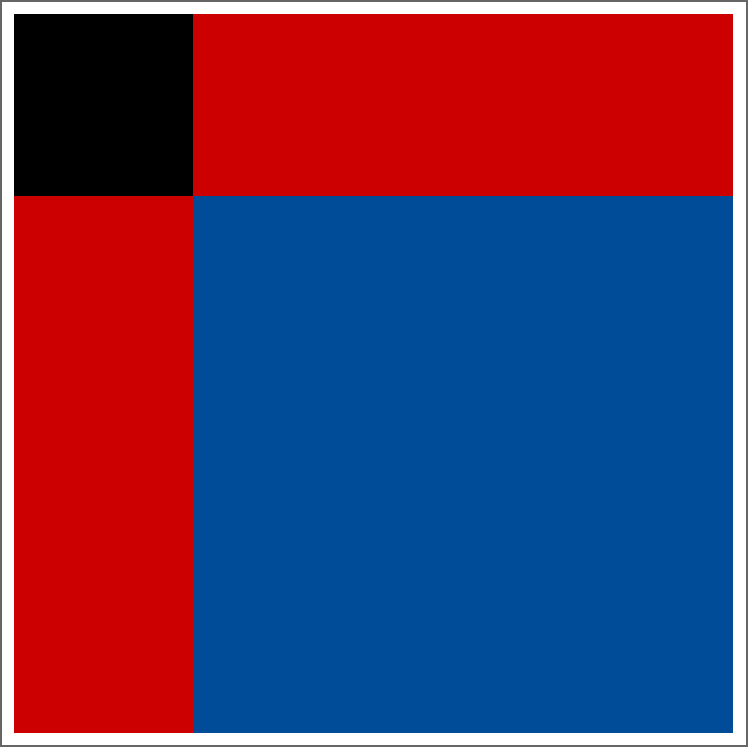
\includegraphics[width=2.2cm]{img-JA/id}  
& \hspace{0.8cm}$\longrightarrow$ 
& 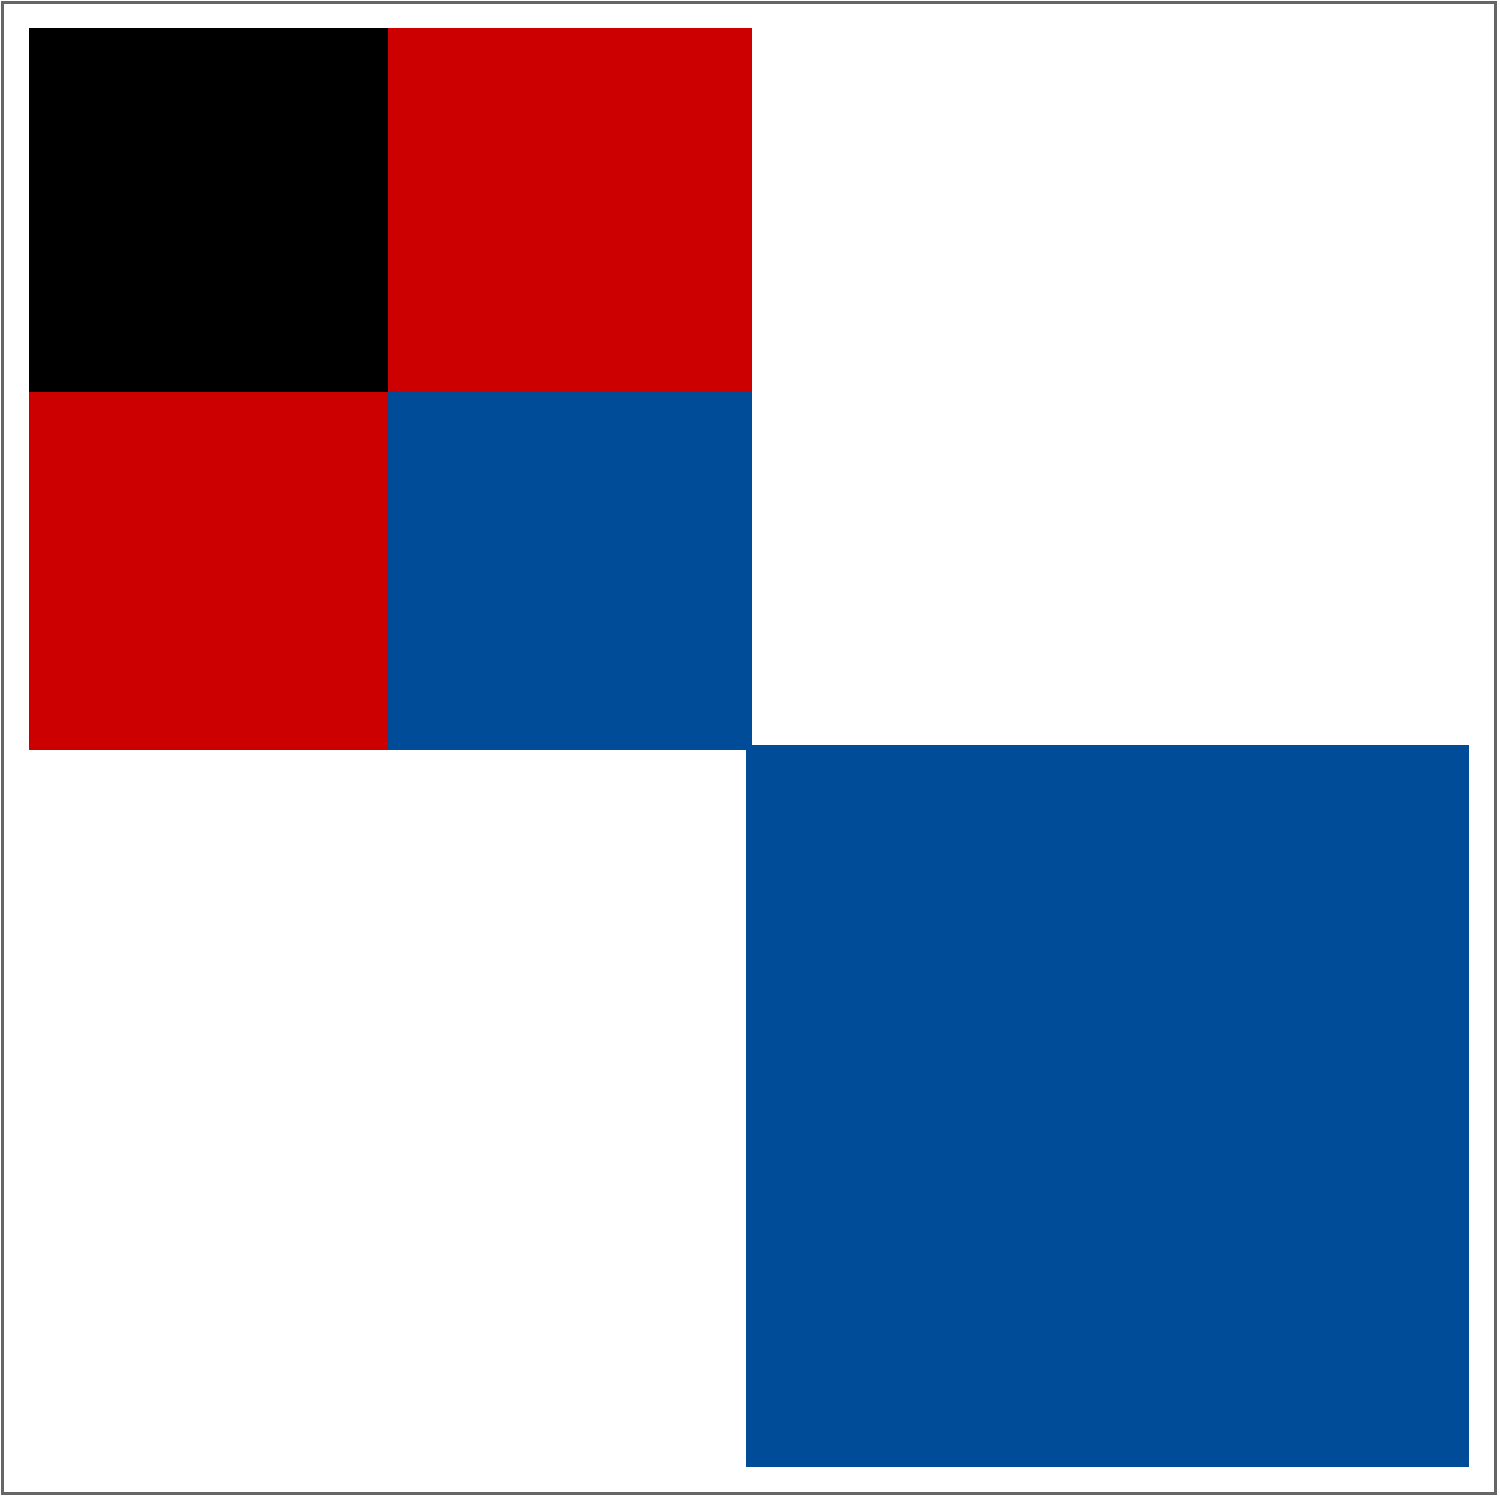
\includegraphics[width=2.2cm]{img-JA/8comp} 
& \hspace{0.8cm}$\longrightarrow$ 
& 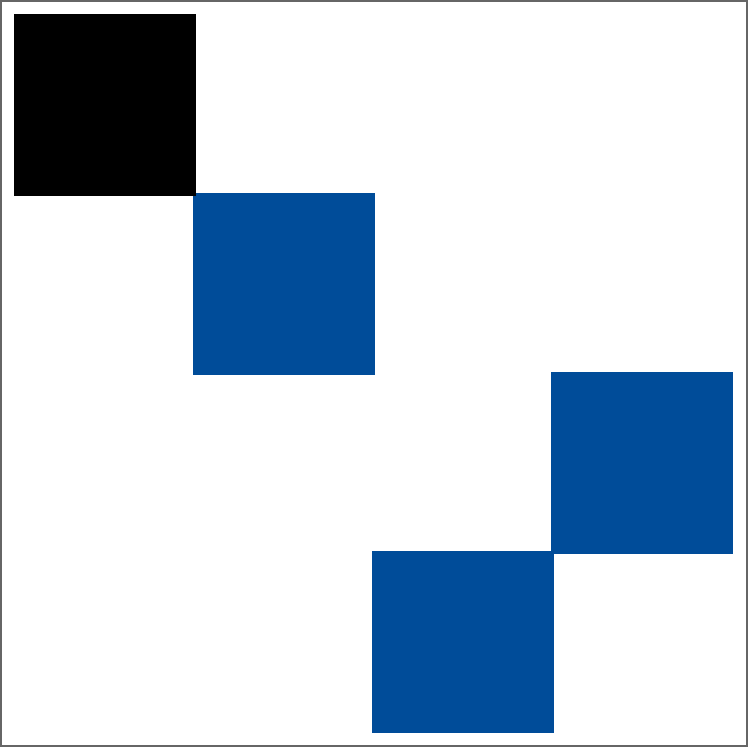
\includegraphics[width=2.2cm]{img-JA/4comp}\\ 
 & 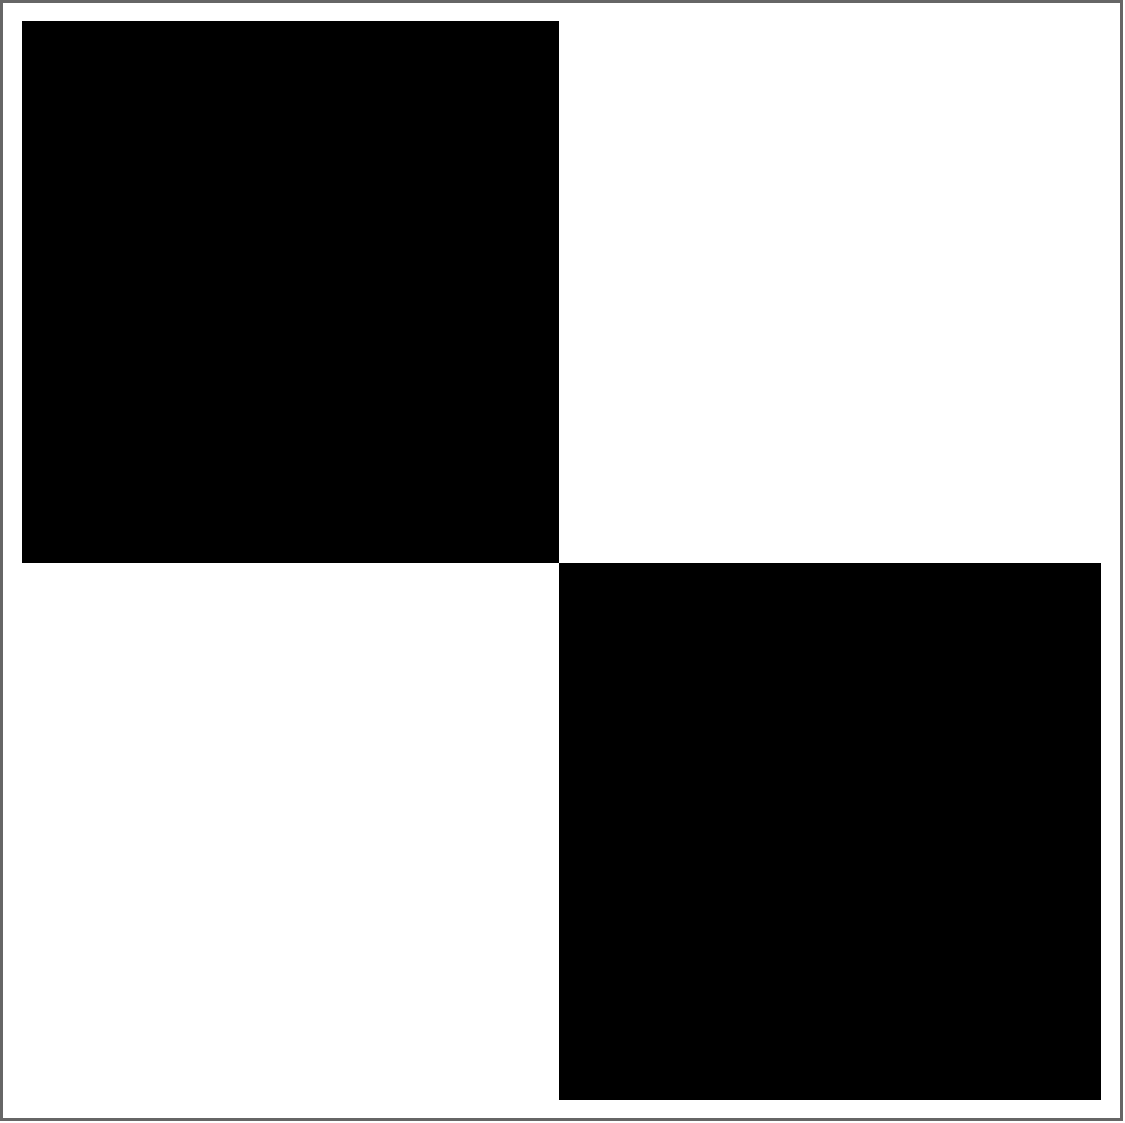
\includegraphics[width=2.2cm]{img-JA/16To8} &  
 & 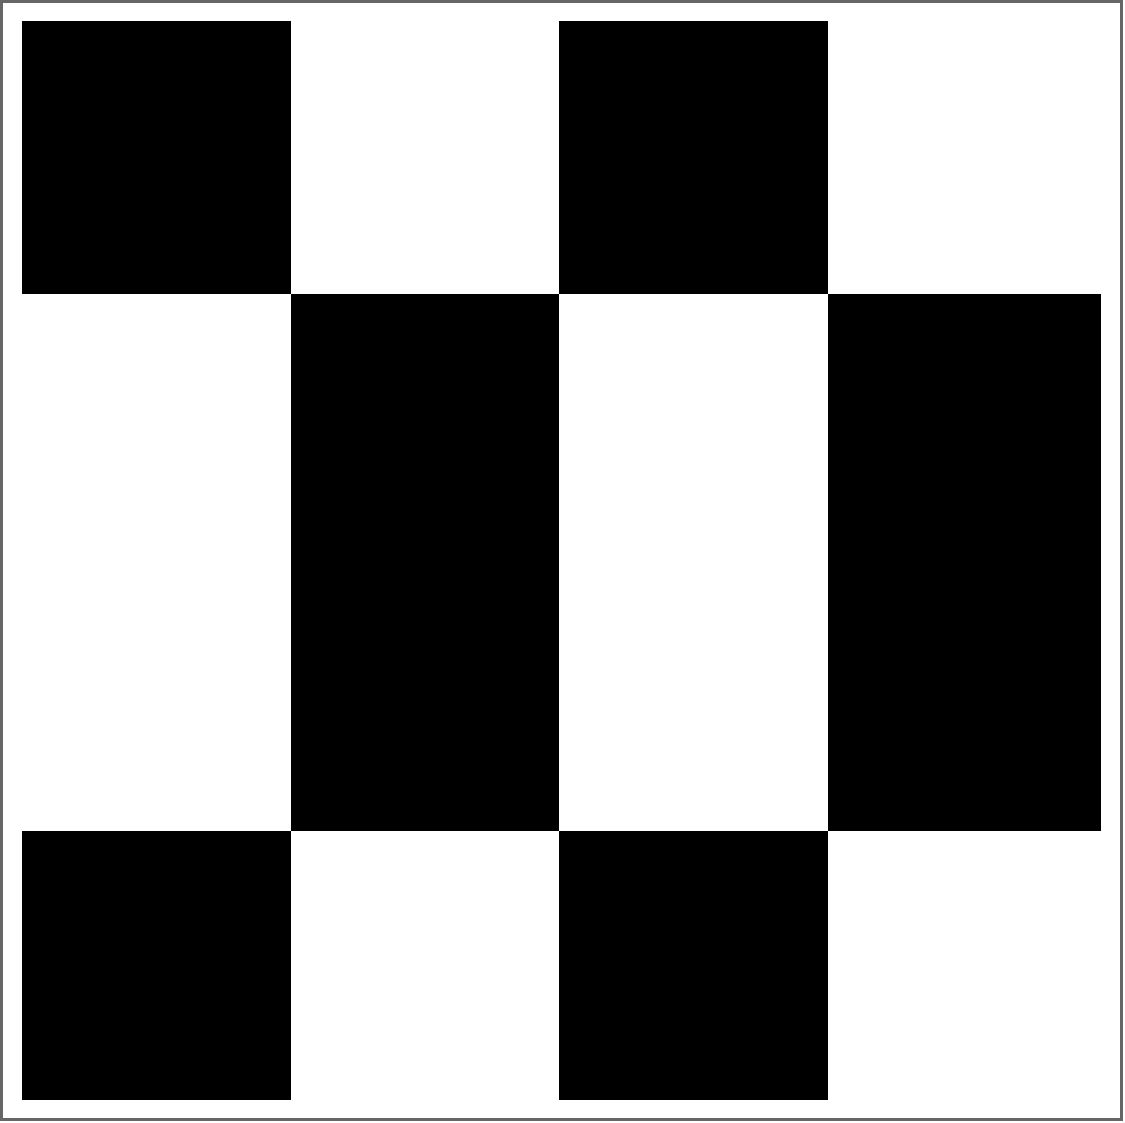
\includegraphics[width=2.2cm]{img-JA/8To4} &\\ 
\end{tabular} 
\end{itemize}


\item \textbf{2 components:}\newline
\begin{itemize}
\item C$_1^2$: $\E_{15}\E_{14}\E_1$\newline
\begin{tabular}{m{2cm} m{2cm} m{2cm} m{2cm} m{2cm} m{2cm} m{2cm}}
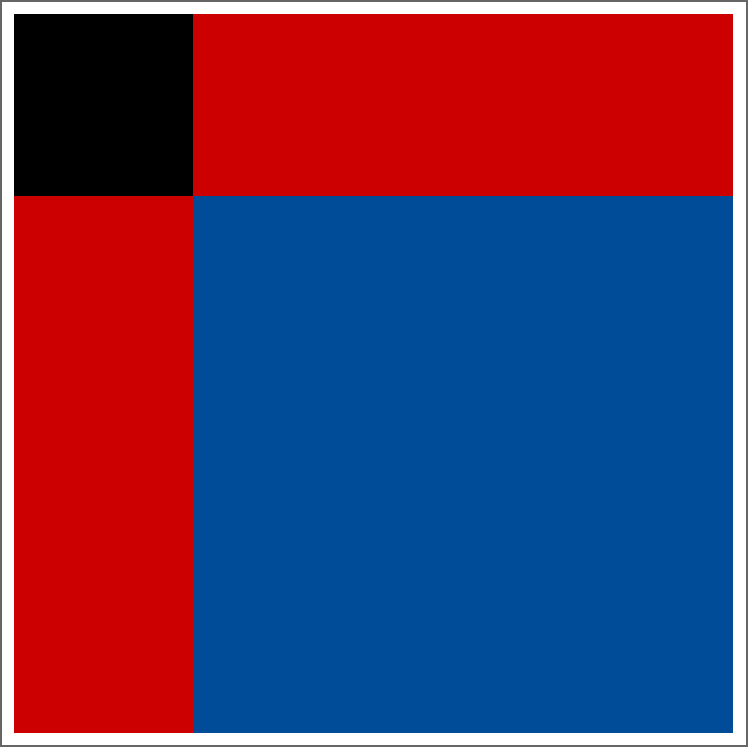
\includegraphics[width=2.2cm]{img-JA/id}  
& \hspace{0.8cm}$\longrightarrow$ 
& 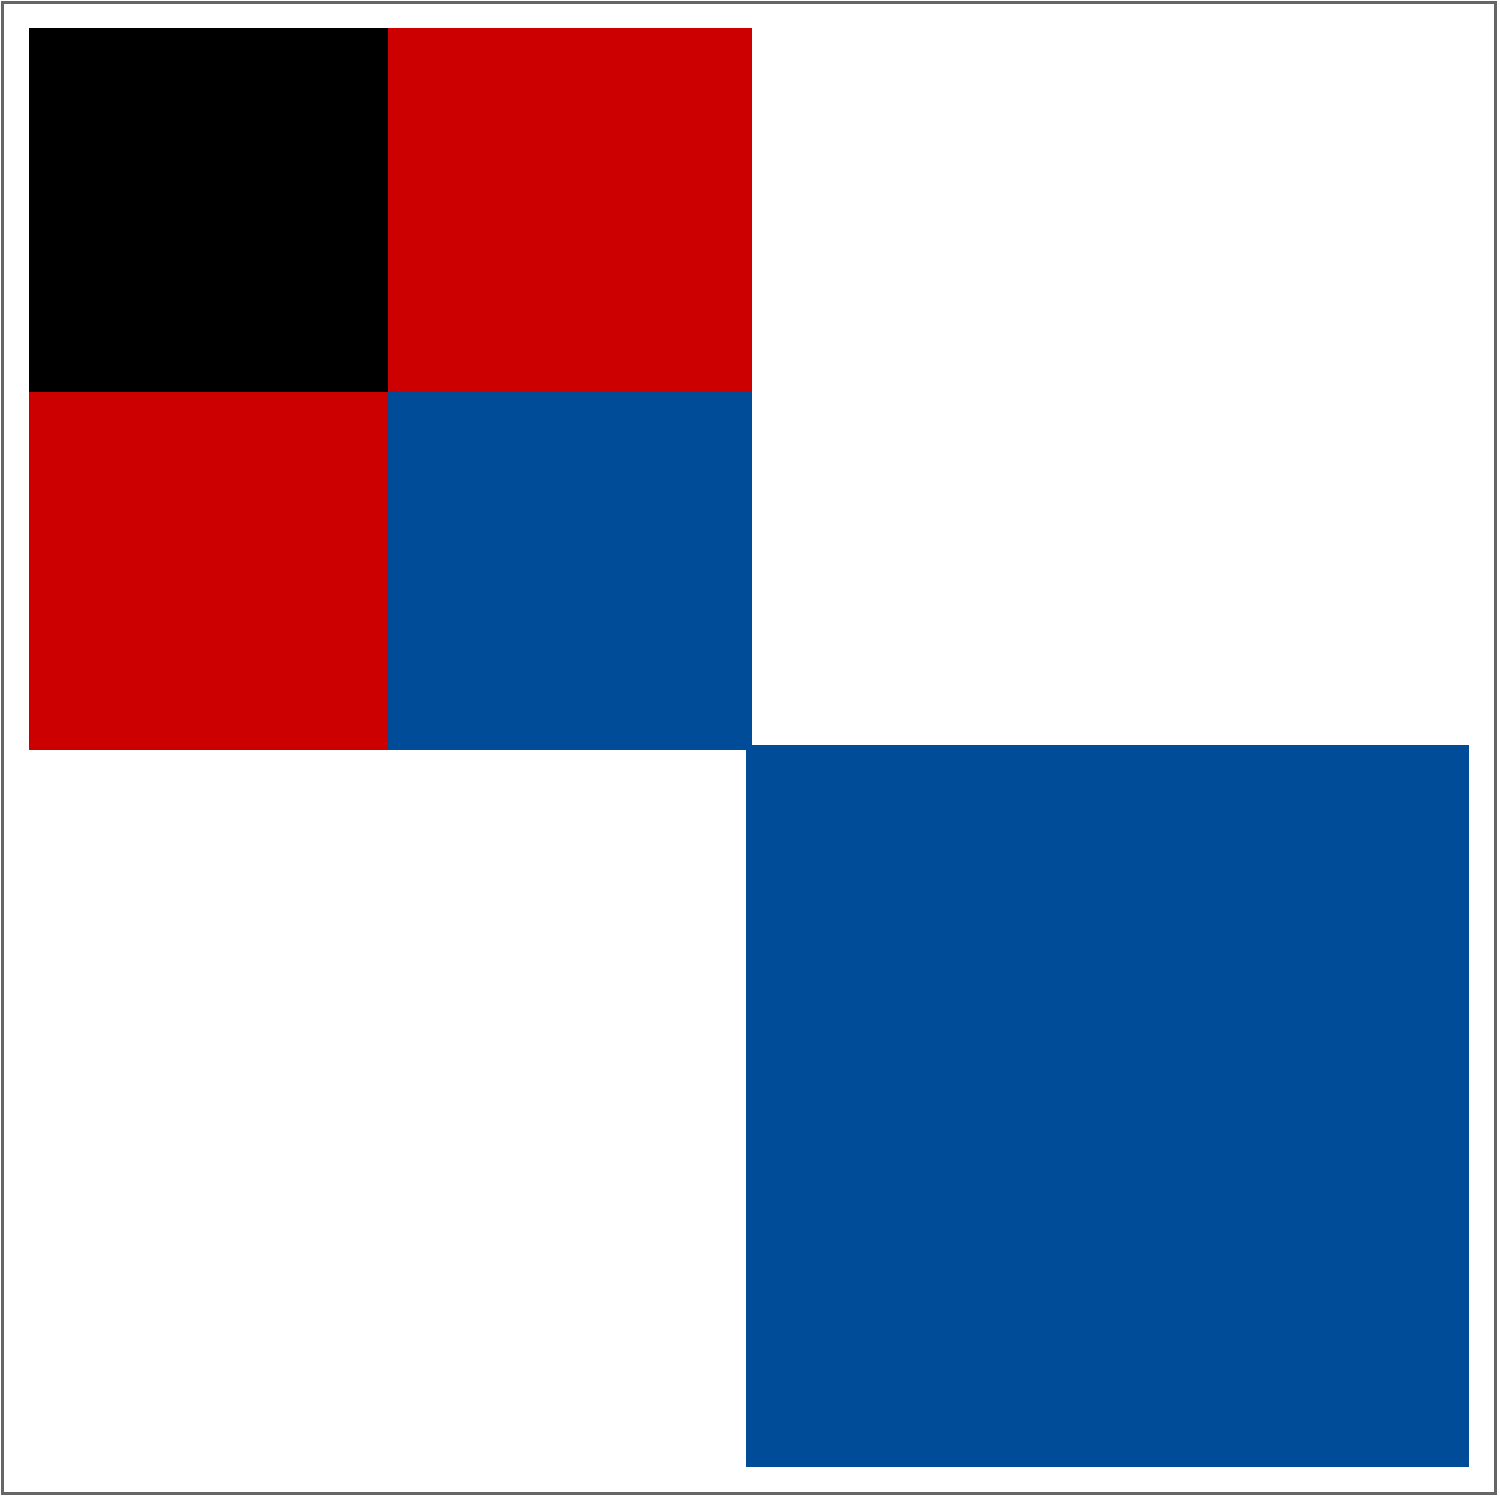
\includegraphics[width=2.2cm]{img-JA/8comp} 
& \hspace{0.8cm}$\longrightarrow$ 
& 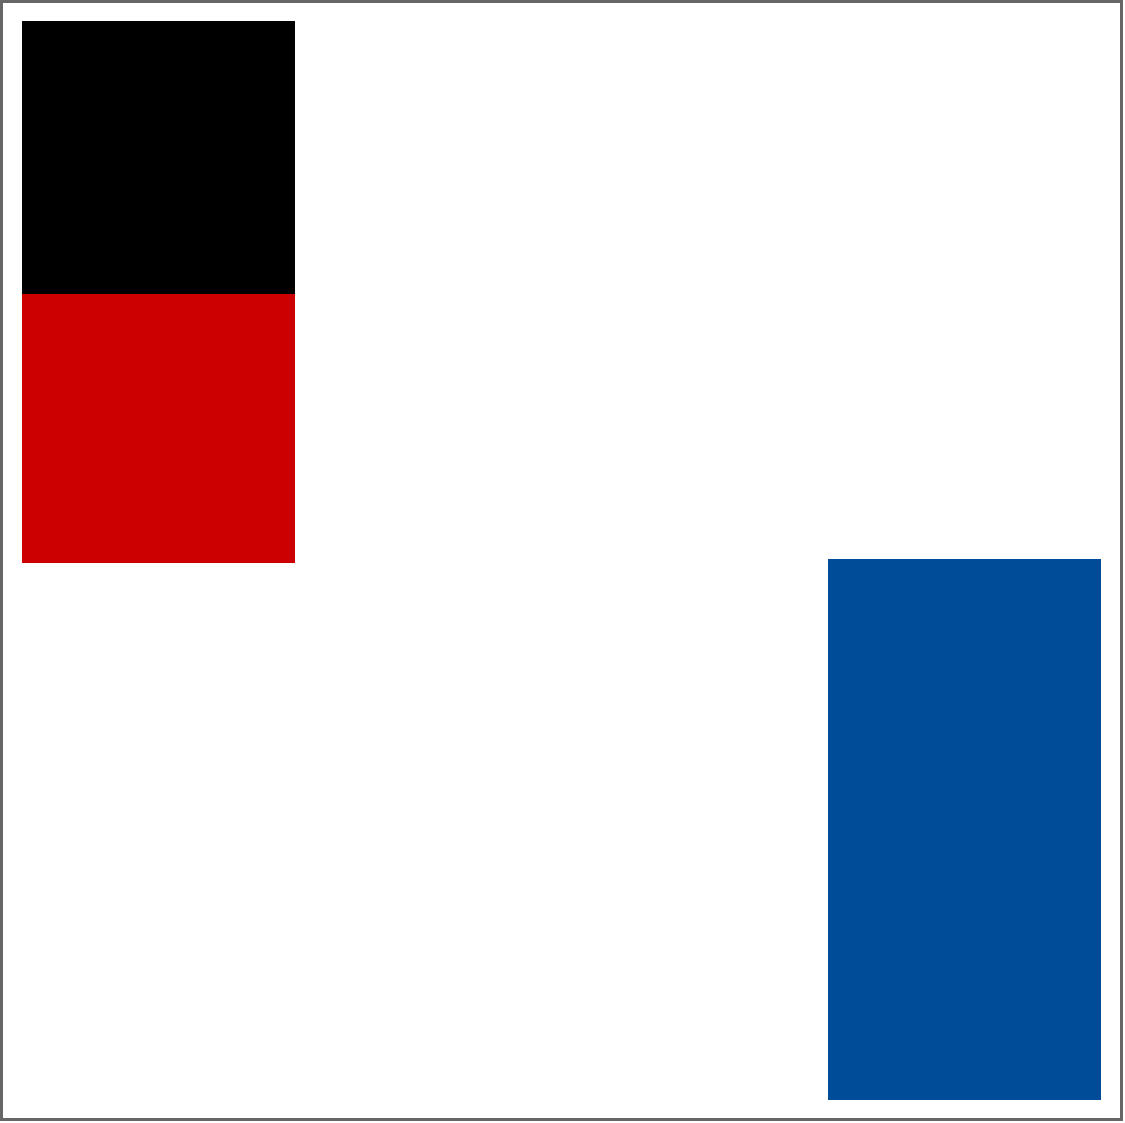
\includegraphics[width=2.2cm]{C43}
& \hspace{0.8cm}$\longrightarrow$ 
& 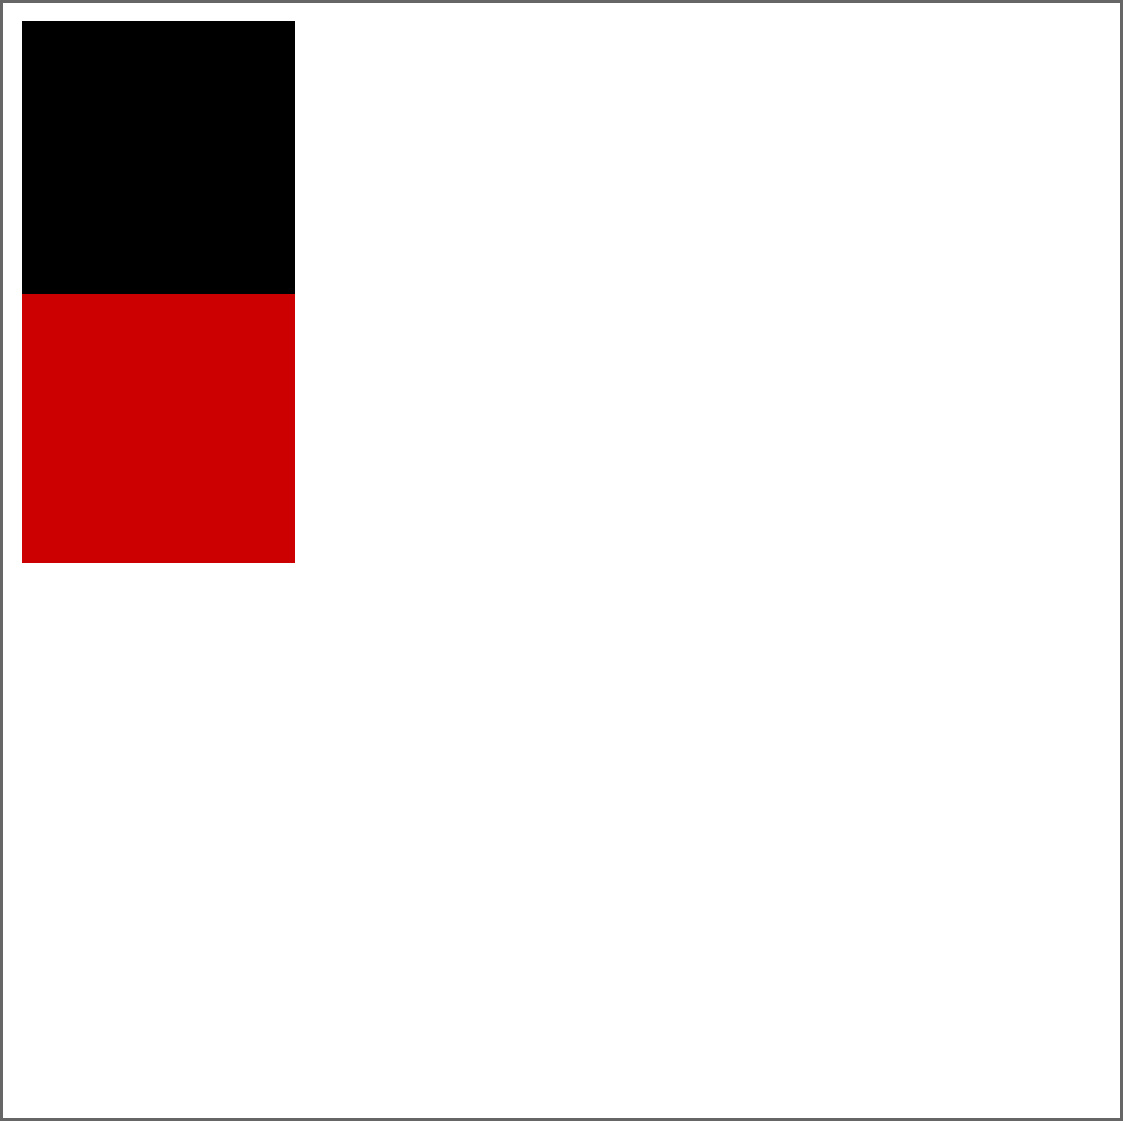
\includegraphics[width=2.2cm]{C21}\\ 
 & 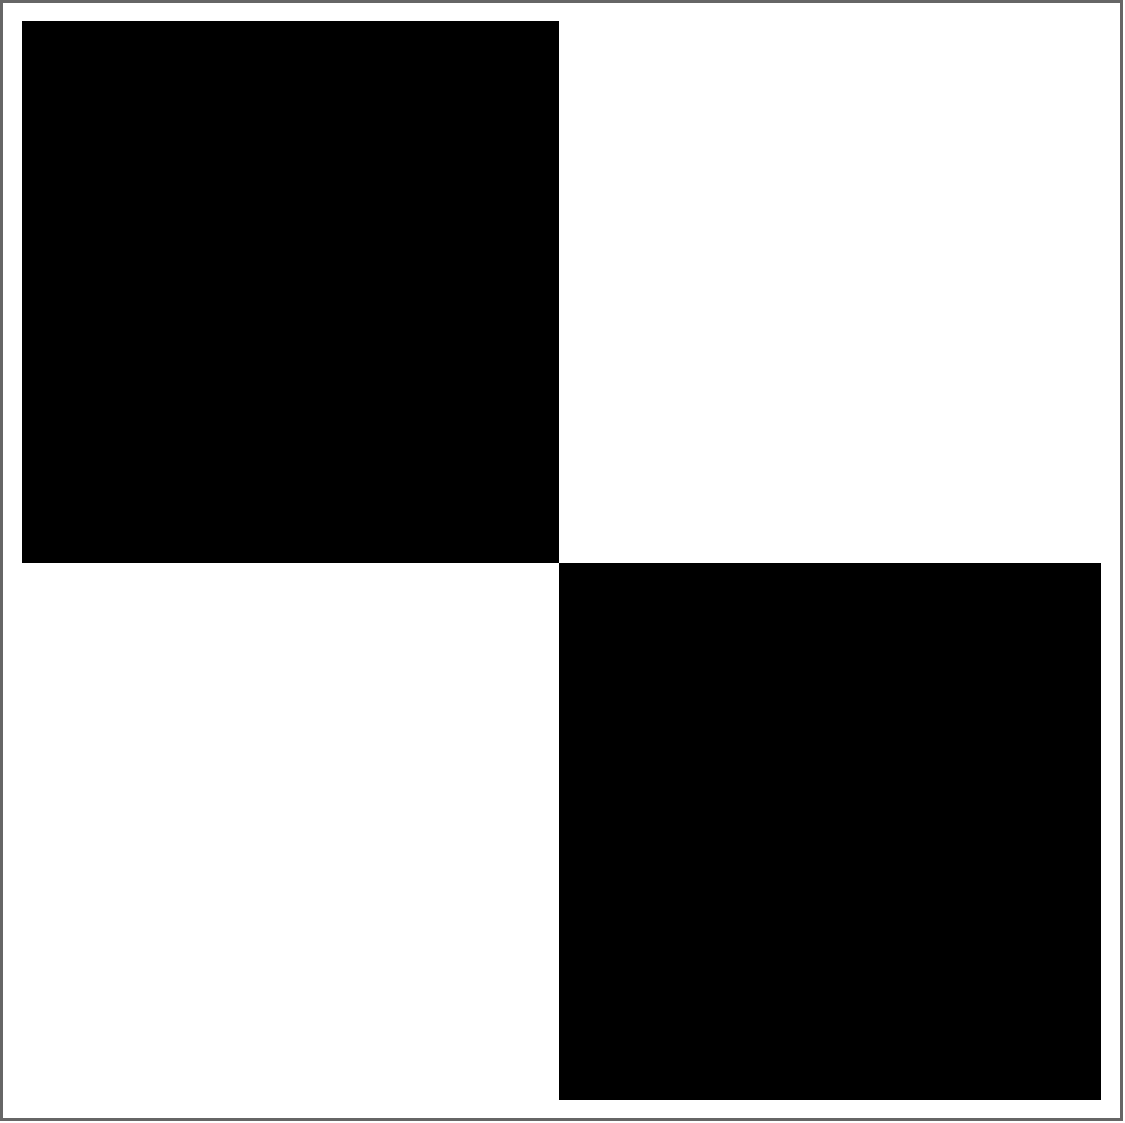
\includegraphics[width=2.2cm]{img-JA/16To8} &  
 & 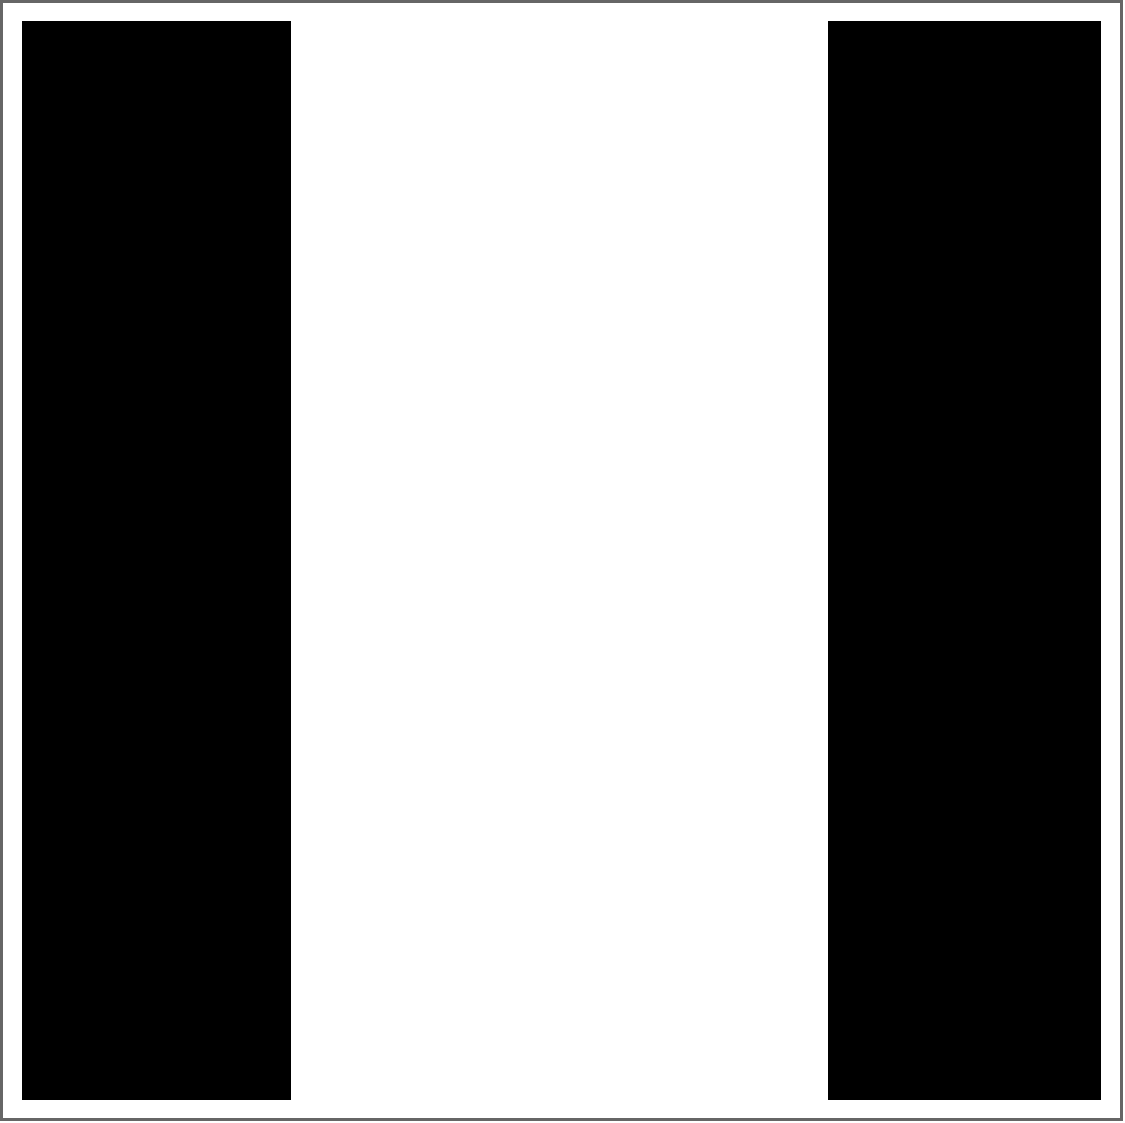
\includegraphics[width=2.2cm]{semefue} &
 & 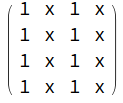
\includegraphics[width=2.2cm]{ruleC81_2} &\\ 
\end{tabular} 

\item C$_2^2$: $\E_6\E_7\E_1$\newline
\begin{tabular}{m{2cm} m{2cm} m{2cm} m{2cm} m{2cm} m{2cm} m{2cm}}
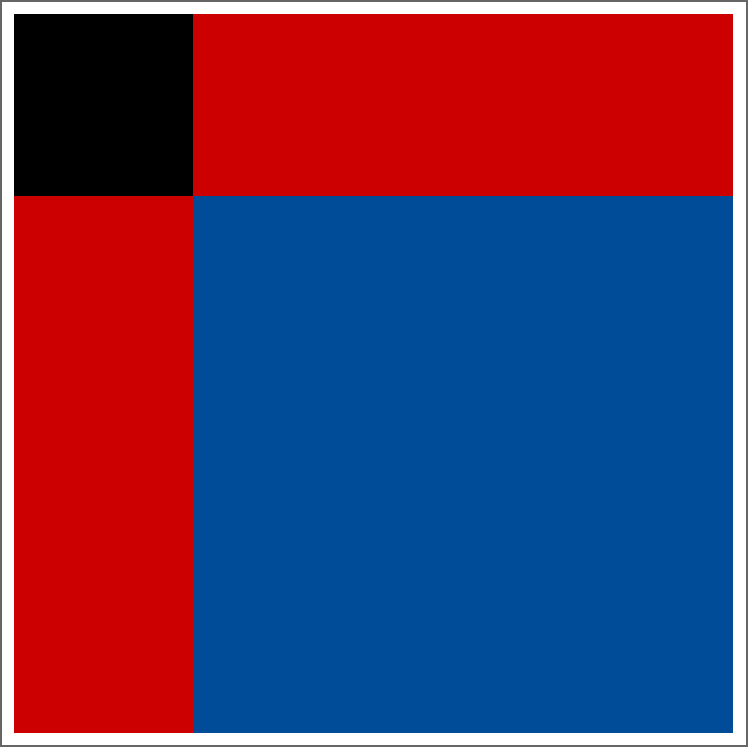
\includegraphics[width=2.2cm]{img-JA/id}  
& \hspace{0.8cm}$\longrightarrow$ 
& 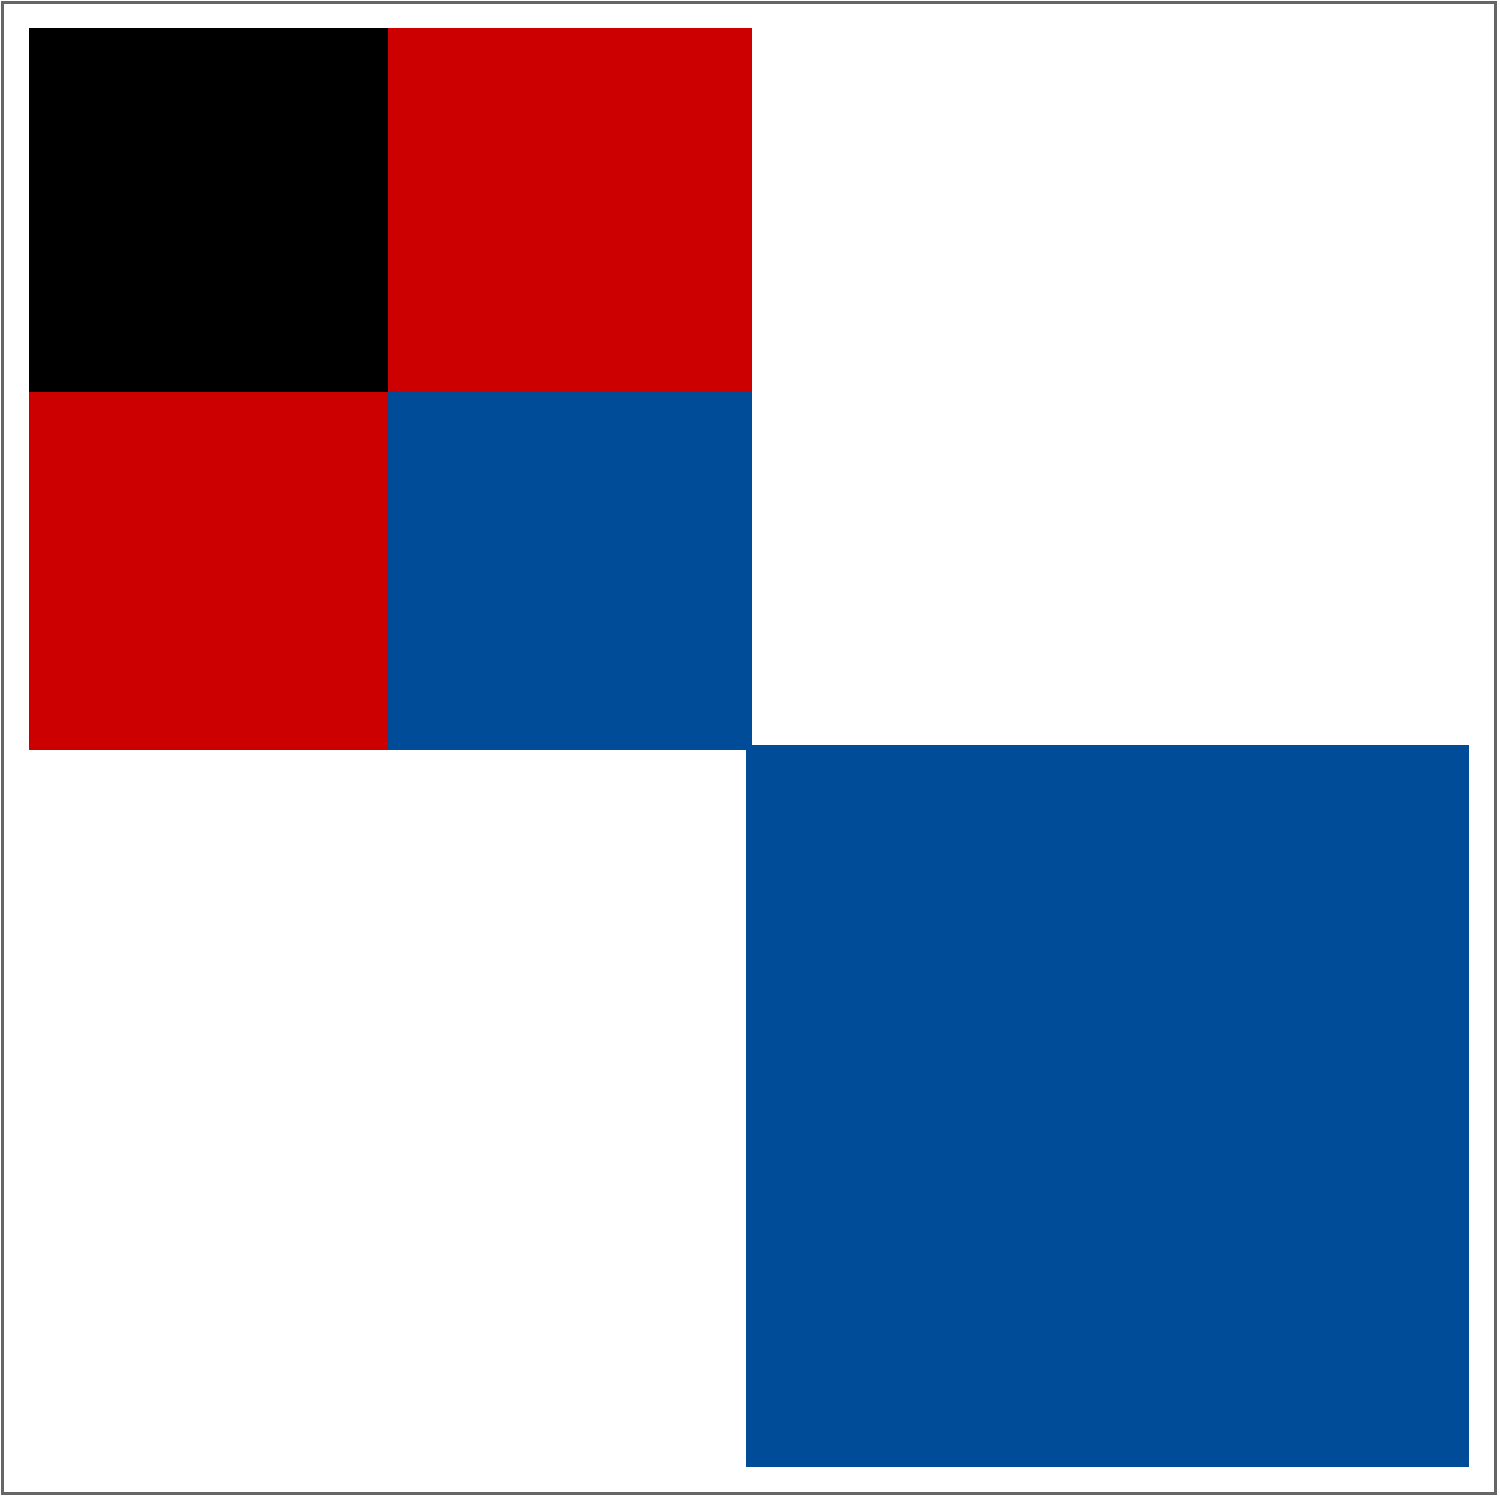
\includegraphics[width=2.2cm]{img-JA/8comp} 
& \hspace{0.8cm}$\longrightarrow$ 
& 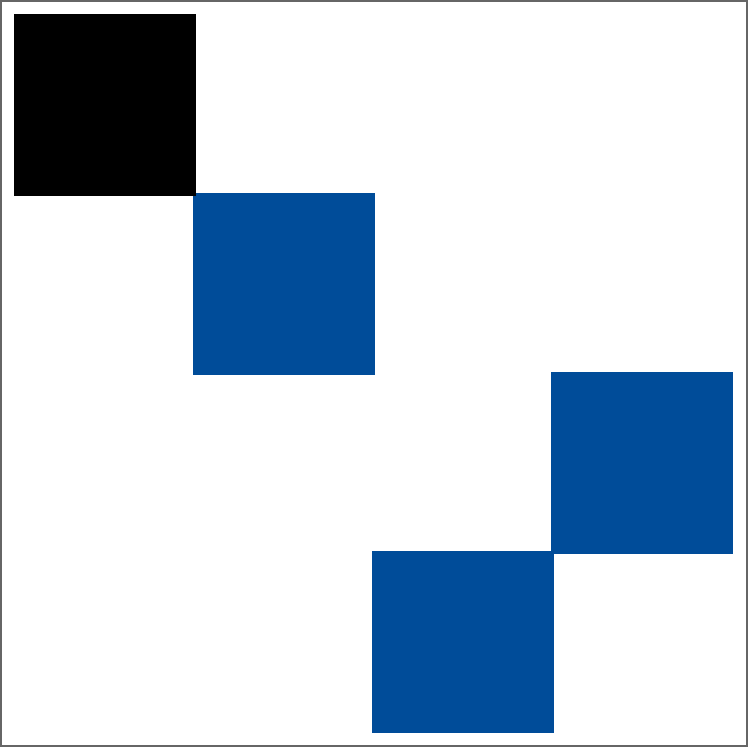
\includegraphics[width=2.2cm]{img-JA/4comp}
& \hspace{0.8cm}$\longrightarrow$ 
& 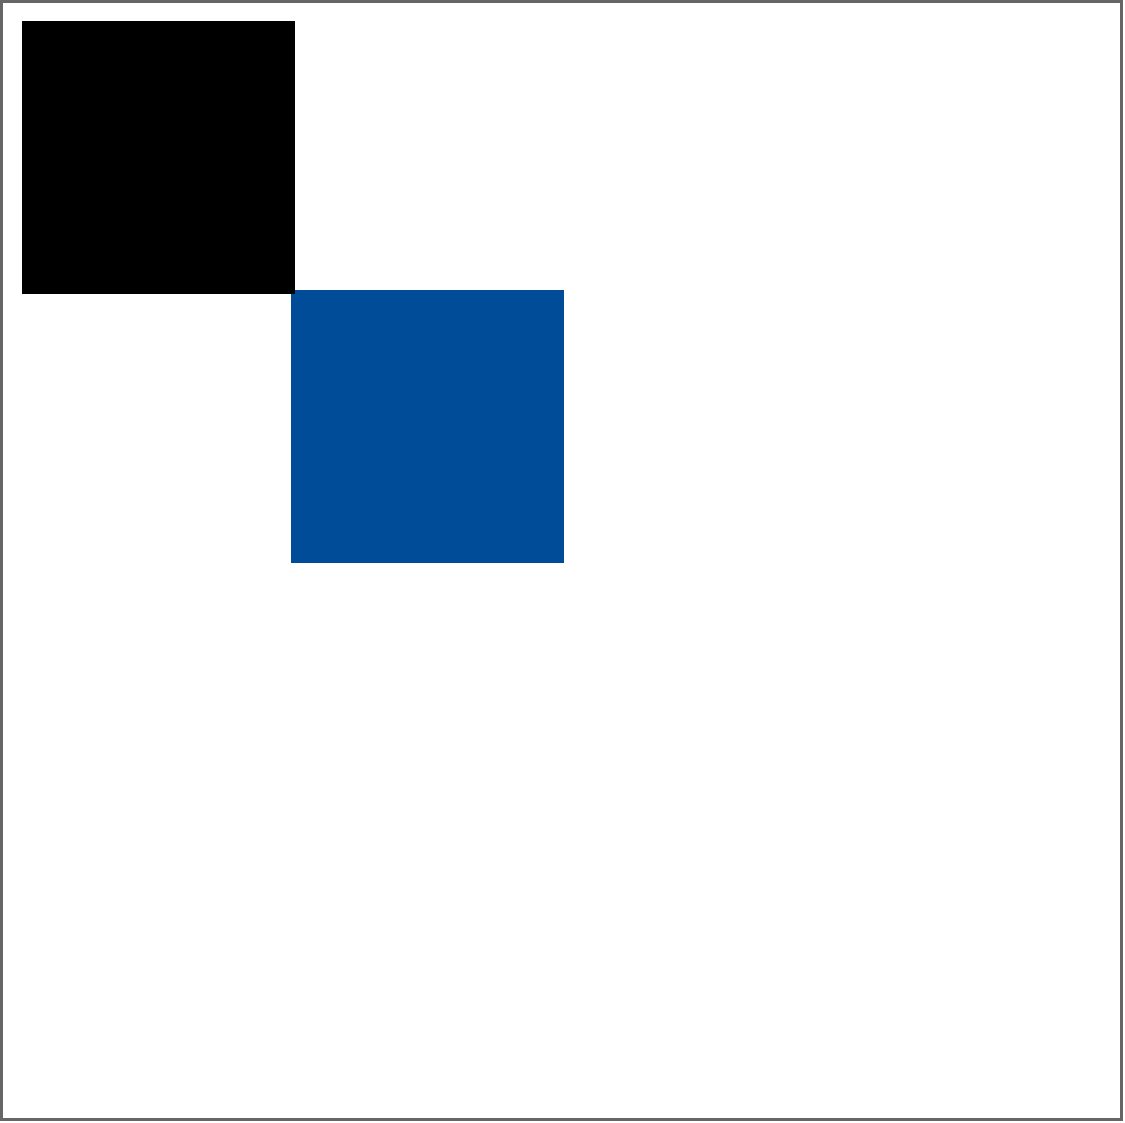
\includegraphics[width=2.2cm]{C22}\\ 
 & 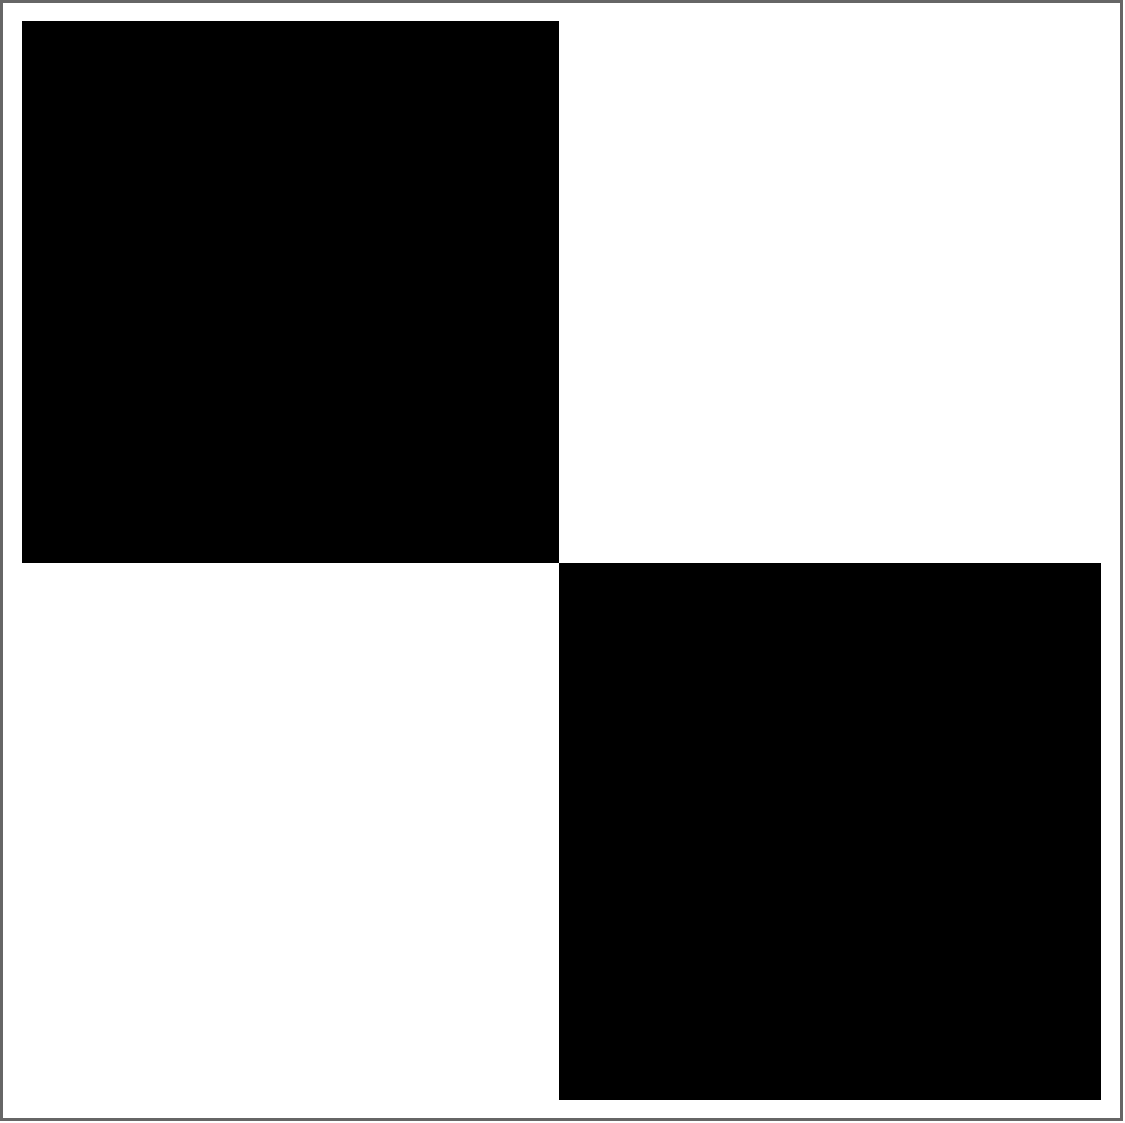
\includegraphics[width=2.2cm]{img-JA/16To8} &  
 & 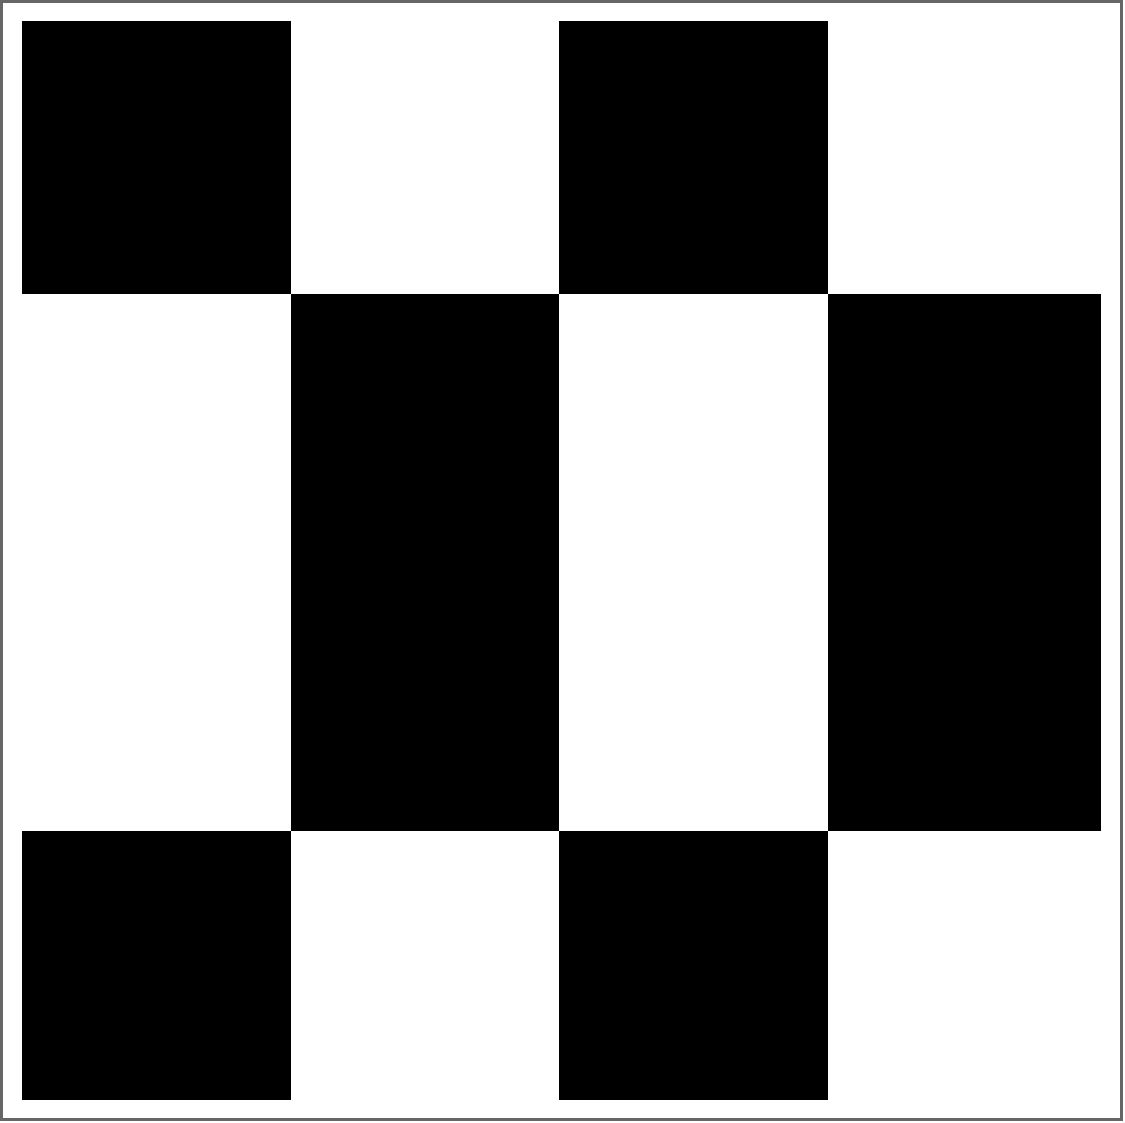
\includegraphics[width=2.2cm]{img-JA/8To4} &
 & 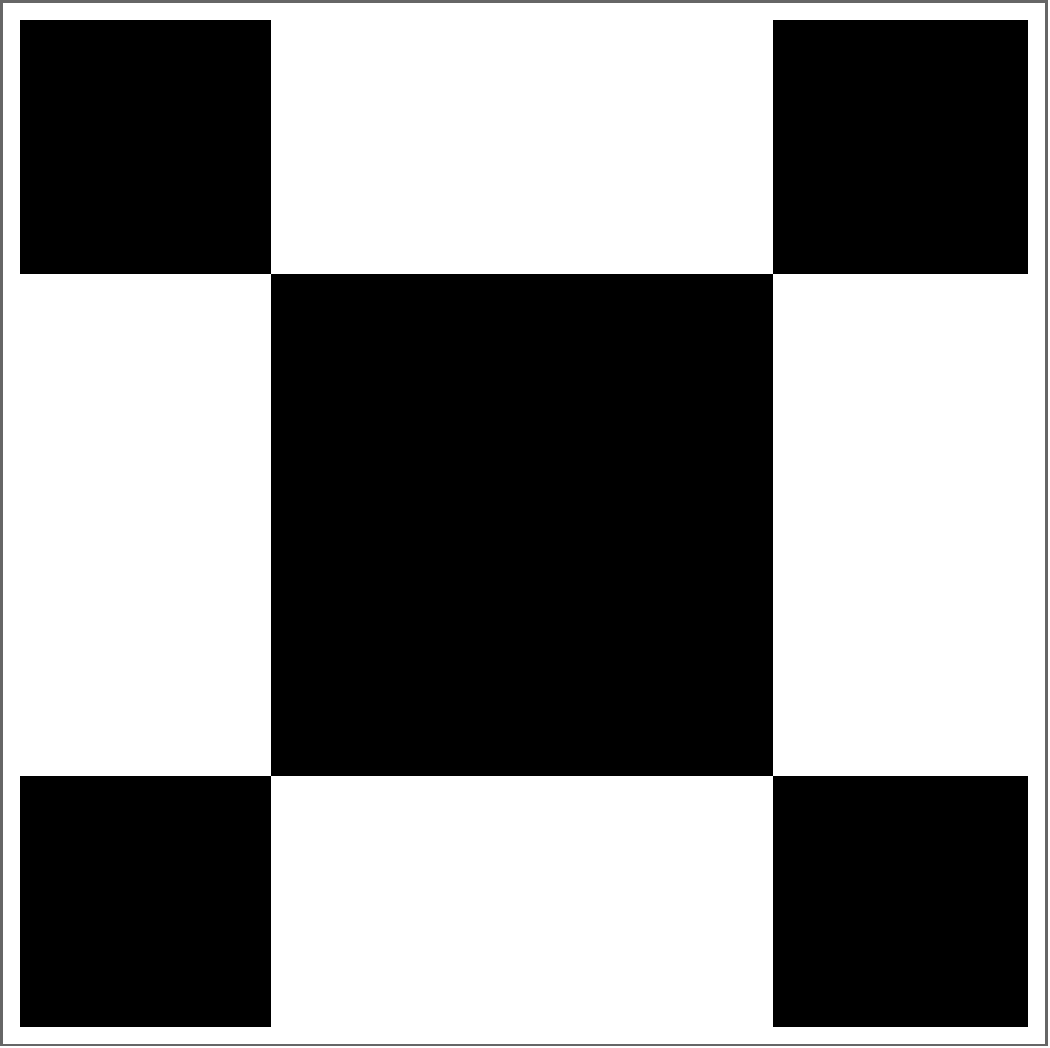
\includegraphics[width=2.2cm]{otroTambien}\\ 
\end{tabular}
\end{itemize}


\pagebreak
\item \textbf{1 component:} $\E_9\E_6\E_7\E_1$\newline
\begin{tabular}{m{2cm} m{2cm} m{2cm}}
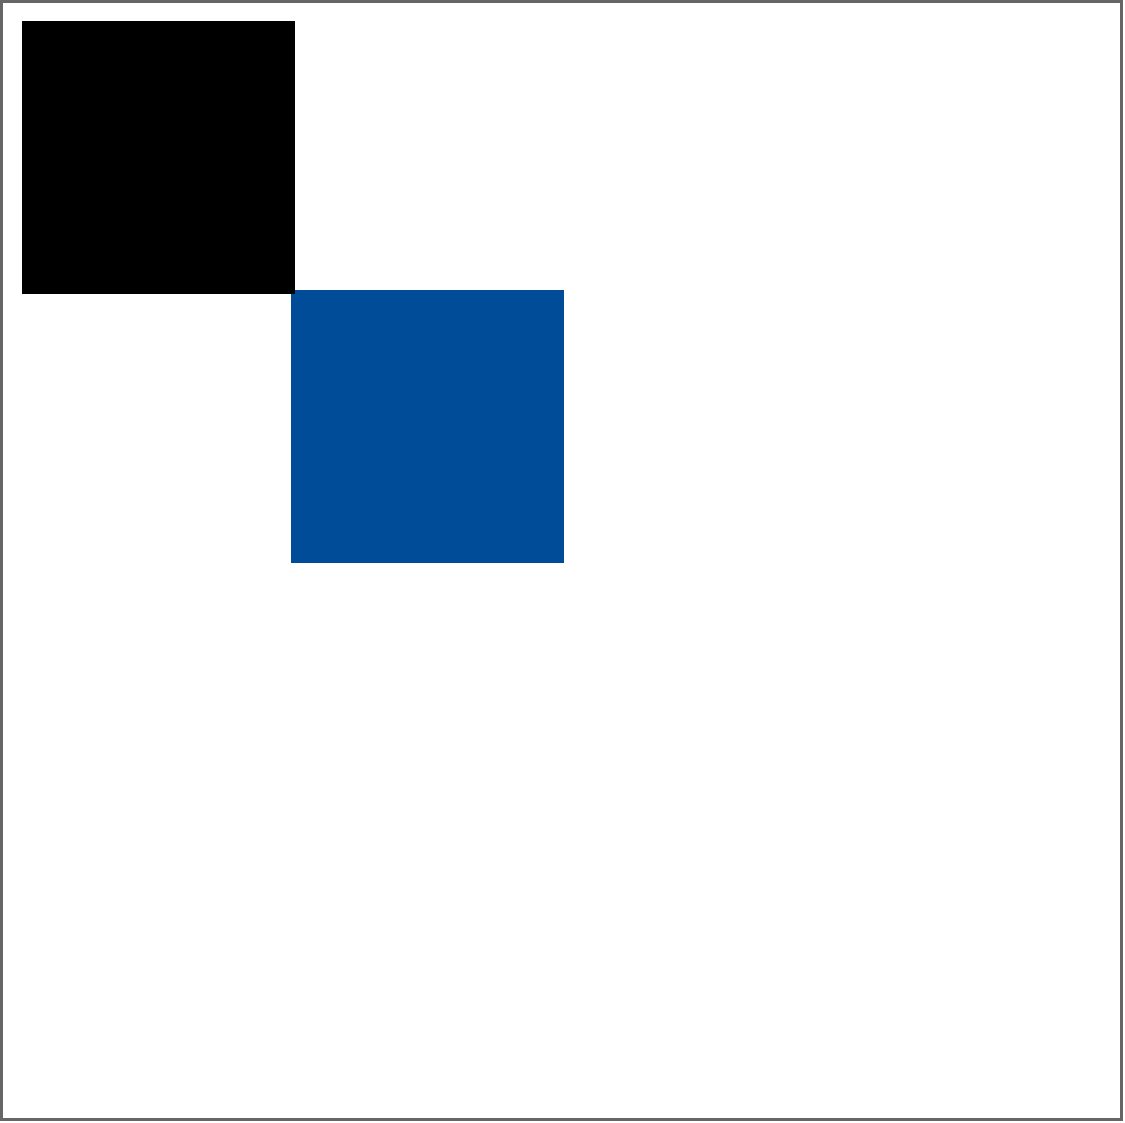
\includegraphics[width=2.2cm]{C22}
& \hspace{0.8cm}$\longrightarrow$ 
& 
\includegraphics[width=2.2cm]{depolarizing} \\ 
 & 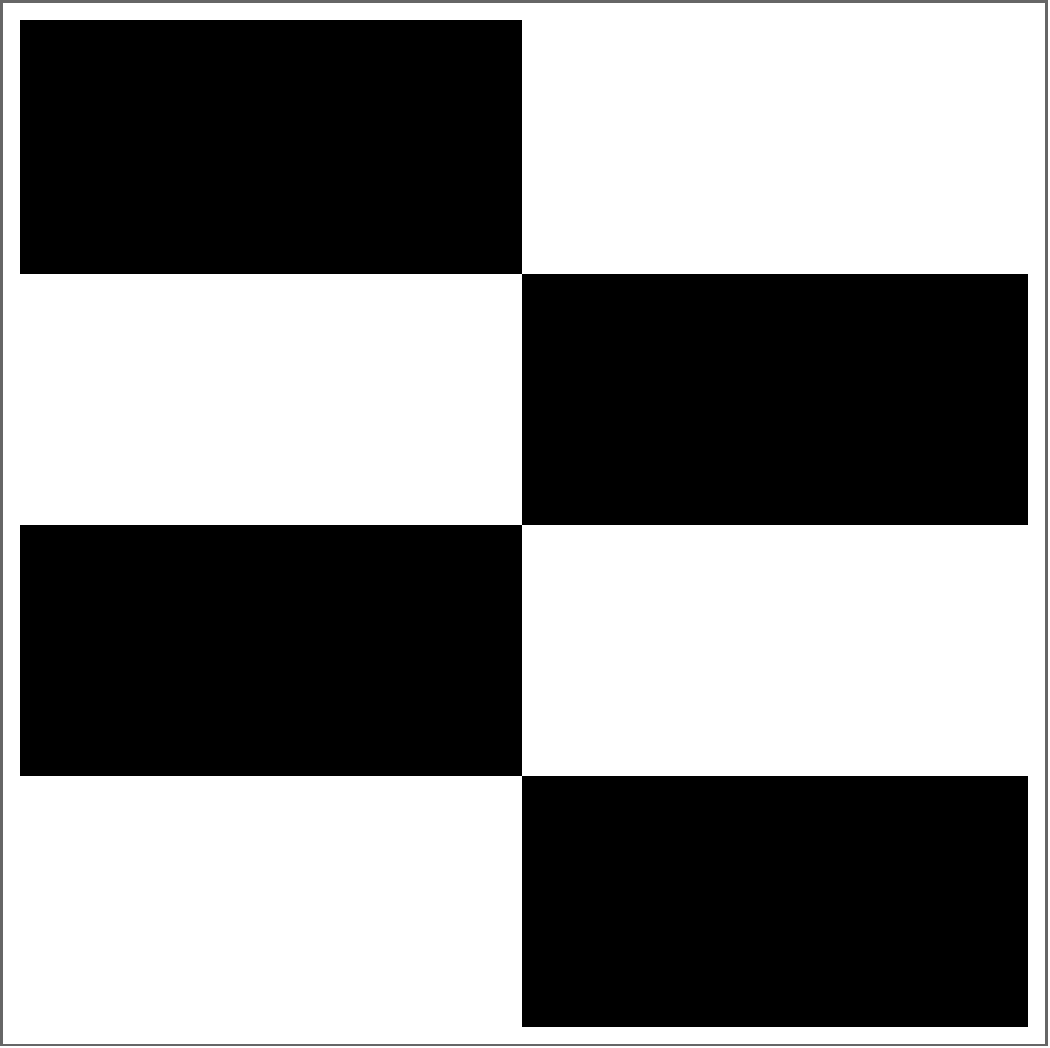
\includegraphics[width=2.2cm]{img-JA/otro} &  \\ 
\end{tabular}
\end{itemize}

\begin{conj}
Only $n$ elements in $\Gamma_n$ are sufficient to generate the 
remaining elements.
\end{conj}
% }}}
\subsection{Numerical Results} % {{{
Hypothesis 1 has strong numerical support. The search for PCE quantum
channels has been done in two different ways:
\begin{enumerate}
\item Using the inequalities in \eqref{eq:inequalities-PCE} to test CP of 
all PCE operations (even the ones that do not follow the power-of-2 rule).
\item Using hypoteshis 1.
\end{enumerate}
Both methods have analyzed the cases of 1, 2, 3 and partially 4 qubits. 
Both of them get the same results. 

\begin{figure}[H]
  \centering
  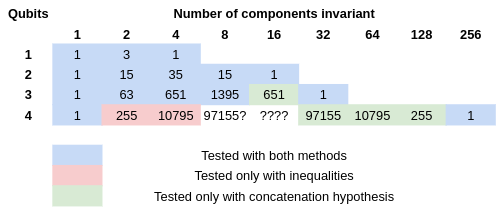
\includegraphics[width=.6\textwidth]{cuadro}
\end{figure}
% }}}
% }}}
\section{Things to do and questions to answer} % {{{
\begin{enumerate}
\item This characterization may explain the power-of-2 rule. 
It is quite obvious (in the figures representation) that the concatenation
always erases half of the number of non-zero components. A proof 
for that is missing.
\item Analytic proof for \eqref{eq:inequalities-PCE}. 
\item Analytic proof that \eqref{eq:PCE-characterization} is necessary 
and sufficient to find all elements in $\PCE{n}$.
\item Analytic proof that taking $-1\to 0$ for $a_k^k$ leads to CP.
I suggest using particle swaps and local basis permutation in order 
to reduce the problem to $n$ inequalities.
\item Find a way to count PCE channels.
\end{enumerate}
% }}}

\section{Progress}
\subsection{An idea to prove equation \eqref{eq:eigvals-PCE}}
A density matrix of 1 qubit in Pauli matrices basis is written as
\begin{align}
\rho=\frac{1}{2}\sum_{i=0}^3r_i\sigma_i,
\end{align}
where $\sigma_i$ are a $2\times2$ identity plus Pauli matrices.
For 2 qubits, in the general case, the density matrix cannot be written as
\begin{align}\label{eq:2qubits-densityM-PauliBasis-separable}
\rho&=\frac{1}{4}\qty(\sum_{i=0}^3r_i\sigma_i
\ot
\sum_{j=0}^3r_j\sigma_j)
\end{align}
because a 2-qubits state is not separable, in general. Therefore, 
the density matrix is written as
\begin{align}
\rho=\frac{1}{4}\sum_{i,j=0}^3r_{i,j}\sigma_{i,j}.
\end{align}
In some sense, expanding 
\eqref{eq:2qubits-densityM-PauliBasis-separable}
\begin{align}
\frac{1}{4}\qty(\sum_{i=0}^3r_i\sigma_i
\ot
\sum_{j=0}^3r_j\sigma_j)
&=\frac{1}{4}\qty(
\1_{4}\ot\1_{4}+\1\ot\sum_{j=1}^3r_j\sigma_j+
\sum_{i=1}^3r_i\sigma_i\ot\1+
\sum_{i=1}^3r_i\sigma_i\ot\sum_{j=1}^3r_j\sigma_j
)
\end{align}
makes us a hint realize that, in the general case, the components
of 2-qubits density matrix in tensor products of Pauli matrices basis are
\begin{align}
r_ir_j&\to r_{i.j},&\ r_i&\to r_{i,0},&\ r_j &\to r_{0,j}.
\end{align}
It follows that $n$-quits density matrix is
\begin{align}
\rho=\frac{1}{2^n}\sum_{j_1,\ldots,j_n=0}^3
r_{j_1,\ldots,j_n}\sigma_{j_1}\ot\ldots\ot\sigma_{j_n},
\end{align}
therefore,
\begin{align}
\label{eq:general-comp-of-density-matrix-in-Pauli-matrices-basis}
r_{j_1}\ldots r_{j_k}\ldots r_{j_n}&\to r_{j_1,\ldots,j_n}, &
r_{j_k}&\to r_{0,\ldots,j_k,\ldots,0},
\end{align}
where 
\begin{align}
r_{j_1}\ldots r_{j_k}\ldots r_{j_n}&\neq r_{j_1,\ldots,j_n}, &
r_{j_k}&\neq r_{0,\ldots,j_k,\ldots,0},
\end{align}

Now, the state $\rho_{\E}$ isomorphic to the Choi matrix $D_{\E}$
(is this written ok?) of a 1-qubit PCE channel~$\E$~is
\begin{align}
\rho_{\E}&=\sum_{i=0}^3\lambda_i \dyad{\sigma_i}{\sigma_i},
\end{align}
where $\ket{\sigma_i}$ are the vectorized $\sigma_i$ and
$\lambda_i$ are (this has been shown analytically)
\begin{align}\label{eq:eigvals-1q-choi}
\lambda_0&=\frac{1}{4}\qty(1+\tau_1+\tau_2+\tau_3), &
\lambda_1&=\frac{1}{4}\qty(1+\tau_1-\tau_2-\tau_3),\nonumber\\
\lambda_2&=\frac{1}{4}\qty(1-\tau_1+\tau_2-\tau_3), &
\lambda_3&=\frac{1}{4}\qty(1-\tau_1-\tau_2+\tau_3).
\end{align}

I claim that, in the same sense of 
\eqref{eq:general-comp-of-density-matrix-in-Pauli-matrices-basis},
the eigenvalues of $\rho_{\E}$ of $n$-qubits PCE quantum channel
$\E$ are of the form
\begin{align}
\lambda_{j_1}\ldots \lambda_{j_k}\ldots \lambda_{j_n}
&\to\lambda_{j_1,\ldots,j_n}, &
\lambda_{j_k}&\to\lambda_{0,\ldots,j_k,\ldots,0},
\end{align}
where $\lambda_k$ are the eigenvalues \eqref{eq:eigvals-1q-choi}.

\section{Number of PCE channels by the ratio of components 
left invariant}
\begin{itemize}
\item 1$/$2 of total components invariant:
\begin{align}
4^n-1
\end{align}

\item 1$/$4 of total components invariant:
\begin{align}
\frac{\binom{4^n-1}{2}}{3},
\end{align}

\item 1$/$8 of total components invariant:
\begin{align}
\frac{\binom{4^n-1}{3}-\binom{4^n-1}{2}/3}{28}
\end{align}

\item 1$/$16 of total components invariant:
\begin{align}
\frac{\binom{4^n-1}{4}-35\qty(\frac{\binom{4^n-1}{3}-\binom{4^n-1}{2}/3}{28})}{840}
\end{align}
\end{itemize}

\begin{table}[h!]
\tiny
\begin{tabular}{llllccccccclll}
{\color[HTML]{FF0000} \textbf{1}} &                       &                           &                                & \multicolumn{1}{l}{} & \multicolumn{1}{l}{}               & \cellcolor[HTML]{FCE5CD}\textbf{1}   & \textbf{3}                             & \textbf{1}                              & \multicolumn{1}{l}{}                    & \multicolumn{1}{l}{}                &                                                       &                                    &                                \\
{\color[HTML]{FF0000} \textbf{2}} &                       &                           &                                & \multicolumn{1}{l}{} & \cellcolor[HTML]{FCE5CD}\textbf{1} & \cellcolor[HTML]{CFE2F3}\textbf{15}  & \cellcolor[HTML]{FCE5CD}\textbf{35}    & \textbf{15}                             & \textbf{1}                              & \multicolumn{1}{l}{}                &                                                       &                                    &                                \\
{\color[HTML]{FF0000} \textbf{3}} &                       &                           &                                & \textbf{1}           & \textbf{63}                        & \cellcolor[HTML]{FCE5CD}\textbf{651} & \cellcolor[HTML]{CFE2F3}\textbf{1,395} & \cellcolor[HTML]{FCE5CD}\textbf{651}    & \textbf{63}                             & \textbf{1}                          &                                                       &                                    &                                \\
{\color[HTML]{FF0000} \textbf{4}} &                       &                           & \multicolumn{1}{c}{\textbf{1}} & \textbf{255}         & \textbf{10,795}                    & 97,155                               & \cellcolor[HTML]{FCE5CD}200,787        & \cellcolor[HTML]{CFE2F3}\textbf{97,155} & \cellcolor[HTML]{FCE5CD}\textbf{10,795} & \textbf{255}                        & \multicolumn{1}{c}{\textbf{1}}                        &                                    &                                \\
{\color[HTML]{FF0000} \textbf{5}} &                       & \multicolumn{1}{c}{1}     & \multicolumn{1}{c}{1,023}      & 174,251              & 6,347,715                          & 53,743,987                           & \multicolumn{1}{l}{}                   & \cellcolor[HTML]{FCE5CD}53,743,987      & \cellcolor[HTML]{CFE2F3}6,347,715       & \cellcolor[HTML]{FCE5CD}174,251     & \multicolumn{1}{c}{\textbf{1,023}}                    & \multicolumn{1}{c}{\textbf{1}}     &                                \\
{\color[HTML]{FF0000} \textbf{6}} & \multicolumn{1}{c}{1} & \multicolumn{1}{c}{4,095} & \multicolumn{1}{c}{2,794,155}  & 408,345,795          & 13,910,980,083                     & \multicolumn{1}{l}{}                 & \multicolumn{1}{l}{}                   & \multicolumn{1}{l}{}                    & \cellcolor[HTML]{FCE5CD}13,910,980,083  & \cellcolor[HTML]{CFE2F3}408,345,795 & \multicolumn{1}{c}{\cellcolor[HTML]{FCE5CD}2,794,155} & \multicolumn{1}{c}{\textbf{4,095}} & \multicolumn{1}{c}{\textbf{1}}
\end{tabular}
\end{table}